% -*- Mode:TeX -*-

%% IMPORTANT: The official thesis specifications are available at:
%%            http://libraries.mit.edu/archives/thesis-specs/
%%
%%            Please verify your thesis' formatting and copyright
%%            assignment before submission. If you notice any
%%            discrepancies between these templates and the 
%%            MIT Libraries' specs, please let us know
%%            by e-mailing thesis@mit.edu

%% The documentclass options along with the pagestyle can be used to generate
%% a technical report, a draft copy, or a regular thesis. You may need to
%% re-specify the pagestyle after you \include cover.tex. For more
%% information, see the first few lines of mitthesis.cls. 

%\documentclass[12pt,vi,twoside]{mitthesis}
%%
%%  If you want your thesis copyright to you instead of MIT, use the
%%  ``vi'' option, as above.
%%
%\documentclass[12pt,twoside,leftblank]{mitthesis}
%%
%% If you want blank pages before new chapters to be labelled ``This
%% Page Intentionally Left Blank'', use the ``leftblank'' option, as
%% above. 

\documentclass[12pt,twoside]{mitthesis}
\usepackage{lgrind}
%% These have been added at the request of the MIT Libraries, because
%% some PDF conversions mess up the ligatures.  -LB, 1/22/2014
\usepackage{cmap}
\usepackage[T1]{fontenc}

%% added by latexdiff

%DIF PREAMBLE EXTENSION ADDED BY LATEXDIFF
%DIF UNDERLINE PREAMBLE %DIF PREAMBLE
\RequirePackage[normalem]{ulem} %DIF PREAMBLE
\RequirePackage{color}\definecolor{RED}{rgb}{1,0,0}\definecolor{BLUE}{rgb}{0,0,1} %DIF PREAMBLE
\providecommand{\DIFadd}[1]{{\protect\color{blue}\uwave{#1}}} %DIF PREAMBLE
\providecommand{\DIFdel}[1]{{\protect\color{red}\sout{#1}}}                      %DIF PREAMBLE
%DIF SAFE PREAMBLE %DIF PREAMBLE
\providecommand{\DIFaddbegin}{} %DIF PREAMBLE
\providecommand{\DIFaddend}{} %DIF PREAMBLE
\providecommand{\DIFdelbegin}{} %DIF PREAMBLE
\providecommand{\DIFdelend}{} %DIF PREAMBLE
%DIF FLOATSAFE PREAMBLE %DIF PREAMBLE
\providecommand{\DIFaddFL}[1]{\DIFadd{#1}} %DIF PREAMBLE
\providecommand{\DIFdelFL}[1]{\DIFdel{#1}} %DIF PREAMBLE
\providecommand{\DIFaddbeginFL}{} %DIF PREAMBLE
\providecommand{\DIFaddendFL}{} %DIF PREAMBLE
\providecommand{\DIFdelbeginFL}{} %DIF PREAMBLE
\providecommand{\DIFdelendFL}{} %DIF PREAMBLE
%DIF END PREAMBLE EXTENSION ADDED BY LATEXDIFF


%% added by hjvm
\usepackage{amsmath}
\DeclareMathOperator*{\argmax}{argmax}
\DeclareMathOperator*{\argmin}{argmin}

\usepackage{hyperref}
\usepackage[round]{natbib}
\setcitestyle{aysep={}}
\hypersetup{
    colorlinks=true,
    linkcolor=black,
    filecolor=magenta, 
    citecolor = black,
    urlcolor=cyan,
}
\usepackage{booktabs}
\usepackage{graphicx}
\usepackage[normalem]{ulem}
\newcommand{\ra}[1]{\renewcommand{\arraystretch}{#1}}
\usepackage[colorinlistoftodos]{todonotes}

\pagestyle{plain}
\raggedbottom


%% This bit allows you to either specify only the files which you wish to
%% process, or `all' to process all files which you \include.
%% Krishna Sethuraman (1990).

%\typein [\files]{Enter file names to process, (chap1,chap2 ...), or `all' to process all files:}
\def\all{all}
\ifx\files\all \typeout{Including all files.} \else %\typeout{Including only \files.} \includeonly{\files} \fi

\begin{document}

% -*-latex-*-
% 
% For questions, comments, concerns or complaints:
% thesis@mit.edu
% 
%
% $Log: cover.tex,v $
% Revision 1.9  2019/08/06 14:18:15  cmalin
% Replaced sample content with non-specific text.
%
% Revision 1.8  2008/05/13 15:02:15  jdreed
% Degree month is June, not May.  Added note about prevdegrees.
% Arthur Smith's title updated
%
% Revision 1.7  2001/02/08 18:53:16  boojum
% changed some \newpages to \cleardoublepages
%
% Revision 1.6  1999/10/21 14:49:31  boojum
% changed comment referring to documentstyle
%
% Revision 1.5  1999/10/21 14:39:04  boojum
% *** empty log message ***
%
% Revision 1.4  1997/04/18  17:54:10  othomas
% added page numbers on abstract and cover, and made 1 abstract
% page the default rather than 2.  (anne hunter tells me this
% is the new institute standard.)
%
% Revision 1.4  1997/04/18  17:54:10  othomas
% added page numbers on abstract and cover, and made 1 abstract
% page the default rather than 2.  (anne hunter tells me this
% is the new institute standard.)
%
% Revision 1.3  93/05/17  17:06:29  starflt
% Added acknowledgements section (suggested by tompalka)
% 
% Revision 1.2  92/04/22  13:13:13  epeisach
% Fixes for 1991 course 6 requirements
% Phrase "and to grant others the right to do so" has been added to 
% permission clause
% Second copy of abstract is not counted as separate pages so numbering works
% out
% 
% Revision 1.1  92/04/22  13:08:20  epeisach

% NOTE:
% These templates make an effort to conform to the MIT Thesis specifications,
% however the specifications can change. We recommend that you verify the
% layout of your title page with your thesis advisor and/or the MIT 
% Libraries before printing your final copy.
\title{Catch me if you can: BERT tries to Syntax.}

\author{H\'ector Javier V\'azquez Mart\'inez}
% If you wish to list your previous degrees on the cover page, use the 
% previous degrees command:
%       \prevdegrees{A.A., Harvard University (1985)}
% You can use the \\ command to list multiple previous degrees
%       \prevdegrees{B.S., University of California (1978) \\
%                    S.M., Massachusetts Institute of Technology (1981)}
\department{Department of Electrical Engineering and Computer Science}

% If the thesis is for two degrees simultaneously, list them both
% separated by \and like this:
% \degree{Doctor of Philosophy \and Master of Science}
\degree{Master of Engineering in Computer Science and Engineering}

% As of the 2007-08 academic year, valid degree months are September, 
% February, or June.  The default is June.
\degreemonth{February}
\degreeyear{2021}
\thesisdate{January 15, 2021}

%% By default, the thesis will be copyrighted to MIT.  If you need to copyright
%% the thesis to yourself, just specify the `vi' documentclass option.  If for
%% some reason you want to exactly specify the copyright notice text, you can
%% use the \copyrightnoticetext command.  
%\copyrightnoticetext{\copyright IBM, 1990.  Do not open till Xmas.}

% If there is more than one supervisor, use the \supervisor command
% once for each.
\supervisor{Robert C. Berwick}{Professor}

% This is the department committee chairman, not the thesis committee
% chairman.  You should replace this with your Department's Committee
% Chairman.
\chairman{Arthur C. Chairman}{Chairman, Department Committee on Graduate Theses}

% Make the titlepage based on the above information.  If you need
% something special and can't use the standard form, you can specify
% the exact text of the titlepage yourself.  Put it in a titlepage
% environment and leave blank lines where you want vertical space.
% The spaces will be adjusted to fill the entire page.  The dotted
% lines for the signatures are made with the \signature command.
\maketitle

% The abstractpage environment sets up everything on the page except
% the text itself.  The title and other header material are put at the
% top of the page, and the supervisors are listed at the bottom.  A
% new page is begun both before and after.  Of course, an abstract may
% be more than one page itself.  If you need more control over the
% format of the page, you can use the abstract environment, which puts
% the word "Abstract" at the beginning and single spaces its text.

%% You can either \input (*not* \include) your abstract file, or you can put
%% the text of the abstract directly between the \begin{abstractpage} and
%% \end{abstractpage} commands.

% First copy: start a new page, and save the page number.
\cleardoublepage
% Uncomment the next line if you do NOT want a page number on your
% abstract and acknowledgments pages.
% \pagestyle{empty}
\setcounter{savepage}{\thepage}
\begin{abstractpage}
% $Log: abstract.tex,v $
% Revision 1.1  93/05/14  14:56:25  starflt
% Initial revision
% 
% Revision 1.1  90/05/04  10:41:01  lwvanels
% Initial revision
% 
%
%% The text of your abstract and nothing else (other than comments) goes here.
%% It will be single-spaced and the rest of the text that is supposed to go on
%% the abstract page will be generated by the abstractpage environment.  This
%% file should be \input (not \include 'd) from cover.tex.

In order to effectively assess Knowledge of Language (KoL) for any statistically-based Language Model (LM), one must develop a test that is first comprehensive in its coverage of linguistic phenomena; second backed by statistically-vetted human judgement data; and third, tests LMs' ability to track human gradient sentence acceptability judgements.  Presently, most studies of KoL on LMs have focused on at most two of these three requirements at a time.  This thesis takes steps toward a test of KoL that meets all three requirements by proposing the LI-Adger dataset: a comprehensive collection of 519 sentence types spanning the field of generative grammar, accompanied by attested and replicable human acceptability judgements for each of the 4177 sentences in the dataset, and complemented by the Acceptability Delta Criterion (ADC), an evaluation metric that enforces the gradience of acceptability by testing whether LMs can track the human data.

To validate this proposal, this thesis conducts a series of case studies with Bidirectional Encoder Representations from Transformers (Devlin et al. 2018).  It first confirms the loss of statistical power caused by treating sentence acceptability as a categorical metric by benchmarking three BERT models fine-tuned using the Corpus of Linguistic Acceptability (CoLA; Warstadt \& Bowman, 2019) on the comprehensive LI-Adger dataset.  We find that although the BERT models achieve approximately 94\% correct classification of the minimal pairs in the dataset, a trigram model trained using the British National Corpus by Sprouse et al. 2018, is able to perform similarly well (75\%).  Adopting the ADC immediately reveals that neither model is able to track the gradience of acceptability across minimal pairs: both BERT and the trigram model only score approximately 30\% of the minimal pairs correctly.  Additionally, we demonstrate how the ADC rewards gradience by benchmarking the default BERT model using \textit{pseudo log-likelihood} (PLL) scores, which raises its score to 38\% correct prediction of all minimal pairs.

This thesis thus identifies the need for an evaluation metric that tests KoL via gradient acceptability over the course of two case studies with BERT and proposes the ADC in response.  We verify the effectiveness of the ADC using the LI-Adger dataset, a representative collection of 4177 sentences forming 2394 unique minimal pairs each backed by replicable and statistically powerful human judgement data.  Taken together, this thesis proposes and provides the three necessary requirements for the comprehensive linguistic analysis and test of the Human KoL exhibited LMs that is currently missing in the field of Computational Linguistics.
\end{abstractpage}

% Additional copy: start a new page, and reset the page number.  This way,
% the second copy of the abstract is not counted as separate pages.
% Uncomment the next 6 lines if you need two copies of the abstract
% page.
% \setcounter{page}{\thesavepage}
% \begin{abstractpage}
% % $Log: abstract.tex,v $
% Revision 1.1  93/05/14  14:56:25  starflt
% Initial revision
% 
% Revision 1.1  90/05/04  10:41:01  lwvanels
% Initial revision
% 
%
%% The text of your abstract and nothing else (other than comments) goes here.
%% It will be single-spaced and the rest of the text that is supposed to go on
%% the abstract page will be generated by the abstractpage environment.  This
%% file should be \input (not \include 'd) from cover.tex.

In order to effectively assess Knowledge of Language (KoL) for any statistically-based Language Model (LM), one must develop a test that is first comprehensive in its coverage of linguistic phenomena; second backed by statistically-vetted human judgement data; and third, tests LMs' ability to track human gradient sentence acceptability judgements.  Presently, most studies of KoL on LMs have focused on at most two of these three requirements at a time.  This thesis takes steps toward a test of KoL that meets all three requirements by proposing the LI-Adger dataset: a comprehensive collection of 519 sentence types spanning the field of generative grammar, accompanied by attested and replicable human acceptability judgements for each of the 4177 sentences in the dataset, and complemented by the Acceptability Delta Criterion (ADC), an evaluation metric that enforces the gradience of acceptability by testing whether LMs can track the human data.

To validate this proposal, this thesis conducts a series of case studies with Bidirectional Encoder Representations from Transformers (Devlin et al. 2018).  It first confirms the loss of statistical power caused by treating sentence acceptability as a categorical metric by benchmarking three BERT models fine-tuned using the Corpus of Linguistic Acceptability (CoLA; Warstadt \& Bowman, 2019) on the comprehensive LI-Adger dataset.  We find that although the BERT models achieve approximately 94\% correct classification of the minimal pairs in the dataset, a trigram model trained using the British National Corpus by Sprouse et al. 2018, is able to perform similarly well (75\%).  Adopting the ADC immediately reveals that neither model is able to track the gradience of acceptability across minimal pairs: both BERT and the trigram model only score approximately 30\% of the minimal pairs correctly.  Additionally, we demonstrate how the ADC rewards gradience by benchmarking the default BERT model using \textit{pseudo log-likelihood} (PLL) scores, which raises its score to 38\% correct prediction of all minimal pairs.

This thesis thus identifies the need for an evaluation metric that tests KoL via gradient acceptability over the course of two case studies with BERT and proposes the ADC in response.  We verify the effectiveness of the ADC using the LI-Adger dataset, a representative collection of 4177 sentences forming 2394 unique minimal pairs each backed by replicable and statistically powerful human judgement data.  Taken together, this thesis proposes and provides the three necessary requirements for the comprehensive linguistic analysis and test of the Human KoL exhibited LMs that is currently missing in the field of Computational Linguistics.
% \end{abstractpage}

\cleardoublepage

\section*{Acknowledgments}

This is the acknowledgements section. You should replace this with your
own acknowledgements.

%%%%%%%%%%%%%%%%%%%%%%%%%%%%%%%%%%%%%%%%%%%%%%%%%%%%%%%%%%%%%%%%%%%%%%
% -*-latex-*-

% Some departments (e.g. 5) require an additional signature page.  See
% signature.tex for more information and uncomment the following line if
% applicable.
% % -*- Mode:TeX -*-
%
% Some departments (e.g. Chemistry) require an additional cover page
% with signatures of the thesis committee.  Please check with your
% thesis advisor or other appropriate person to determine if such a 
% page is required for your thesis.  
%
% If you choose not to use the "titlepage" environment, a \newpage
% commands, and several \vspace{\fill} commands may be necessary to
% achieve the required spacing.  The \signature command is defined in
% the "mitthesis" class
%
% The following sample appears courtesy of Ben Kaduk <kaduk@mit.edu> and
% was used in his June 2012 doctoral thesis in Chemistry. 

\begin{titlepage}
\begin{large}
This doctoral thesis has been examined by a Committee of the Department
of Chemistry as follows:

\signature{Professor Jianshu Cao}{Chairman, Thesis Committee \\
   Professor of Chemistry}

\signature{Professor Troy Van Voorhis}{Thesis Supervisor \\
   Associate Professor of Chemistry}

\signature{Professor Robert W. Field}{Member, Thesis Committee \\
   Haslam and Dewey Professor of Chemistry}
\end{large}
\end{titlepage}


\pagestyle{plain}
  % -*- Mode:TeX -*-
%% This file simply contains the commands that actually generate the table of
%% contents and lists of figures and tables.  You can omit any or all of
%% these files by simply taking out the appropriate command.  For more
%% information on these files, see appendix C.3.3 of the LaTeX manual. 
\tableofcontents
\newpage
\listoffigures
\newpage
\listoftables


\chapter*{Introduction}
\addcontentsline{toc}{chapter}{Introduction}

Assessing the Knowledge of Language (KoL) of statistically-based Language Models (LMs) generally involves assuming some fundamental property or computation occurring in the Human Language Faculty and arguing that a currently poorly understood, statistical, and typically connectionist model, also partakes in the use of that property or computation.  This quickly becomes a problematic task because understanding the Human Language Faculty has been conventionally posed as a problem to be solved at a causal level removed from the algorithmic and computational implementation levels.  Put in more abstract terms, assessing the KoL of a LM requires inferring some abstract operation inside a human black box based on input-output analysis and determining whether a second, statistical black box is somehow also performing the same operation by some other means.  

The issue is made even more challenging by changes in either field that consequently change our assumptions surrounding the Human Language Faculty or the black boxes used in Machine Learning (ML). This, in turn, immediately impacts claims relating the two by some abstract property, linguistic or otherwise, that is required for the evaluation of LMs.  If any concrete progress is to be made when it pertains to KoL in LMs, then the design of the tests we perform and their conclusions must be based on the same empirical data from current input-output analyses of the Human Language Faculty that has subsequently been used to build the linguistic theories that attempt to characterize and explain Human KoL.  

This thesis takes concrete steps toward designing such a test of KoL for LMs by positing the necessary components required to build upon the same bedrock of empirical data as the field of generative grammar in Linguistics.  First, we propose the LI-Adger dataset, a collection of statistically powerful and attested linguistic phenomena representative of the field of Linguistics (\citealt{sprouse2012assessing,sprouse2013comparison}), accompanied by human acceptability judgements in the form of Magnitude Estimation (ME) data.  Altogether, the dataset has an attested maximum False Positive (Type 1 error) rate between 1-12\% and is well above the 80\% threshold for statistical power (<20\% False Negatives, or Type 2 errors) \citep{sprouse2017design}.  The reliability of the LI-Adger dataset is such that, if the linguistic theories were somehow proven to be incorrect and reformulated, it would not be because of the data, but because of incorrect theorizing; any tractable theory of linguistics must account for the empirical phenomena observed in the LI-Adger dataset \citep{sprouse2012assessing}.  To complement this data, we propose the Acceptability Delta Criterion (ADC), a proof of concept metric that enforces the gradience of acceptability in its evaluation of model performance, and adopts the continuous human judgements as the ground-truth labels that LMs must approximate in order to demonstrate KoL.

Our results suggest that, when acceptability is treated as a functionally categorical metric on isolated minimal pairs of sentences as it has been traditionally treated in the literature (\citealp{linzen2016assessing,marvin2018targeted,wilcox2018rnn,warstadt2020can}; among others), the task of determining sentence acceptability fails to properly test for KoL.  Under this relaxed metric, the large, cased version of Bidirectional Encoder Representations from Transformers (BERT$_{\mathrm{large-cased}}$; \citealp{devlin2018bert}) when fine-tuned using the Corpus of Linguistic Acceptability (CoLA; \citealp{warstadt2019neural}) (the model is henceforth referred to as BERT$_\mathrm{CoLA_{large-cased}}$), correctly evaluates 2213 out of 2365 ($\sim$94\%) minimal pairs in the LI-Adger dataset; that is, for those 2213 minimal pairs, BERT$_\mathrm{CoLA_{large-cased}}$ gives a higher score to the sentence in the minimal pair deemed by experts to be the \textit{acceptable} one of the pair.  We will continue to refer to this metric as the BLiMP Criterion, named after the BLiMP dataset \citep{warstadt2019blimp}.  To put the performance of BERT$_\mathrm{CoLA_{large-cased}}$) into perspective, a trigram model using the Syntactic Log-Odds Ratio (SLOR; \citealp{pauls2012large,lau2017grammaticality}) is able to correctly evaluate 1781 out of 2365 ($\sim$75\%) minimal pairs.  Considering the coverage of phenomena in the LI-Adger dataset, we may interpret these results in one of two ways: either metrics such as the BLiMP Criterion lead to statistically underpowered tests with a high rate of false positives, or a basic trigram model using SLOR encodes the KoL necessary to account for 75\% of the phenomena in Linguistics.  We opt for the first interpretation and consider this evidence of a theoretical flaw in the metric itself, not a demonstration of what the models \textit{know} about language.

Adopting the ADC (with $\delta=0.5$), which enforces that LMs' predictions be within a set number of standard deviation units ($\delta$) from the human ME judgements, quickly changes the panorama.  BERT$_\mathrm{CoLA_{large-cased}}$ only correctly evaluates 726 out of 2365 ($\sim$31\%) minimal pairs, whereas the trigram model with SLOR correctly evaluates 712 out of 2365 ($\sim$30\%).  These results imply that, when it comes to tracking the acceptability of sentences across minimal pairs, the KoL encoded in BERT does not go much farther than that of an $N$-gram model.


Here we proceed as follows. First, we attempt to replicate the linguistic analysis of BERT conducted by \citet{warstadt2020can} using the grammatically annotated Corpus of Linguistic Acceptability.  Over the course of this replication, we confirm evidence of underspecification in overparametrized Neural LMs as identified by \citet{d2020underspecification,mccoy2019berts}, among others.  In particular, we observe predictions on the LI-Adger sentences from BERT$_\mathrm{CoLA_{base-uncased}}$, the smallest (i.e. least overparametrized) of the original BERT$_\mathrm{CoLA}$ models, is extremely sensitive to the {\em order} in which the CoLA training sentences are presented, even though overall performance remained relatively unchanged.  We observe this behavior even within the same initialization of the model, where the only difference between two runs is the random seed used to shuffle the training data.  This underspecification takes the form of instability in the LI-Adger test set predictions: sentences predicted as acceptable (1) by BERT with around 90-99\% \textit{confidence} flip to be predicted as unacceptable with a similar magnitude, or vice versa.  We find that over the course of 200 different training orders, 1272 sentences, or roughly 30\% of the sentences in the LI-Adger dataset exhibit this flipping behavior.  We affectionately name this subset of sentences the Acrobatic Sentences.

Given the alarmingly high proportion of acrobatic sentences produced by the predictions from BERT$_\mathrm{CoLA_{base-uncased}}$, we find ourselves obliged to consider successful replication as achieving Matthew's Correlation Coefficient (MCC) scores on the CoLA test set that are \textit{reasonably} close to those reported by \citet{warstadt2019blimp}.  To this end, we select the BERT$_\mathrm{CoLA}$ models with the single best performance on the CoLA out-of-domain test set and further test them using the LI-Adger dataset under the BLiMP Criterion.  Although we find that the BERT$_\mathrm{CoLA}$ models satisfy the BLiMP criterion for roughly 94\% of the minimal pairs, the magnitudes of their predictions do not track the degrees of acceptability exhibited by the gradient human judgements.  

When benchmarking BERT$_\mathrm{CoLA}$ models using the BLiMP criterion, the output of the models is determined by multiplying the final hidden vector ($\vec{h}\in \mathbf{R}^d$) by a weight matrix $W\in \mathbf{R}^{2\mathrm{x}d}$ learned during the fine-tuning phase and taking the softmax of the product, written explicitly in Equation \ref{eqn:softmax}.
\begin{equation}
    \mathrm{softmax}(\vec{x}) = \frac{e^{x_i}}{\sum_{j=0}^{j=K}e^{x_j}}
    \label{eqn:softmax}
\end{equation}
The final output of the BERT$_\mathrm{CoLA}$ models ($out$) is then computed by taking argmax of the two-dimensional vector resulting from the softmax, as expressed in Equation \ref{eqn:argmax_softmax}, thus yielding the final categorical 1/0 prediction.
\begin{equation}
    out = \argmax\bigg[\mathrm{softmax}(Wh)\bigg]
    \label{eqn:argmax_softmax}
\end{equation}
However, in order to improve the BERT$_\mathrm{CoLA}$ models' performance apriori before applying the ADC, we adopt the labels $\pm1$ instead of 1/0 and scale the predicted labels by the output of the final softmax classification head in Equation \ref{eqn:softmax}.  Now we have an approximate method of knowing when the BERT$_\mathrm{CoLA}$ models consider a sentence completely acceptable ($\sim$0.95), completely unacceptable ($\sim$ -0.95), and anything in between.  We confirm we do not lose any information because the categorical labels are recovered by taking the sign of the new output.  The delta in the BERT$_\mathrm{CoLA_{large-cased}}$ model's acceptability scores across minimal pairs using this more gradient output metric only weakly correlates with the human judgements ($\sim$0.349, $p$<0.0001).  For reference, conducting the same analysis with the SLOR scores of a trigram model trained on the British National Corpus \citep{sprouse2018colorless} yields almost the same Pearson's correlation coefficient ($\sim$0.333, $p$<0.0001).

The above analyses by nature warrant further controls.  For one, we are uncertain of what information--semantic, syntactic or otherwise--might be introduced into the BERT models by the CoLA training set itself, as opposed to already being present in their pretrained representations.  Additionally, training a linear classifier on top of the BERT models' embeddings very rarely yields a softmax output of less than 0.95, meaning most predictions were around either 0.99 or -0.99.  In spite of BERT's claimed KoL, expecting gradience from the resulting BERT$_\mathrm{CoLA}$ after fine-tuning using the categorical labels could be viewed as unfair to the model due to its lack of access to gradient data.  We believe this is a fair expectation because we do not have access to categorically labeled raw linguistic input during language acquisition, and we are ultimately probing the LMs for Human KoL.  Regardless, we repeat the analyses on the out-of-the-box version of BERT (BERT$_\mathrm{MLM}$).  We obtain \textit{pseudo-log-likelihood} (PLL) scores from BERT$_\mathrm{MLM}$ by performing a variant of a Cloze test in which we sequentially mask each word in a given sentence and retrieve the probability of the originally masked token as predicted by BERT$_\mathrm{MLM}$ (\citealp{wang2019bert,shin2019effective,salazar2020} ).\footnote{We are fully aware that Jacob Devlin himself has said that BERT is not a language model and recommended against this sequential masked language modeling procedure (See the \href{https://github.com/google-research/bert/issues/35}{original issue on the Google Research GitHub repository}).  We point readers to \citet{salazar2020}, who report BERT$_\mathrm{MLM}$ beats the state-of-the-art GPT-2 on BLiMP \citep{warstadt2019blimp} when using PLL scores.}  In this task, the total PLL of a sentence $s_i$ of length $n$ is the sum total of the log-likelihood score of each of its tokens $[w_0,...,w_n]$, which can be expressed as:
\begin{equation}
    \mathrm{PPL(s_i)} = \sum^{n}_{j=0} \mathrm{log}(P(w_j|w_0,...,w_{j-1},w_{j+1},...w_n))
    \label{eqn:pseudo_log_likelihood}
\end{equation}
We find that this objective only slightly improves performance under the ADC: scoring 890 out of 2365 ($\sim$38\%) minimal pairs with $\delta = 0.5$, as well as slightly improving the correlation with the human judgement deltas across minimal pairs ($\sim$0.384, $p$<0.0001).  

Given the results of these analyses, the contributions of this thesis are threefold.  First, it highlights the importance of interpreting sentence acceptability as a gradient metric and demonstrates how exhibiting such gradience is a prerequisite to attributing any KoL to a LM.  Secondly, it proposes the Acceptability Delta Criterion as a proof of concept measurement that enforces the gradience of acceptability in its evaluation of performance and adopts continuous human judgements as the ground-truth labels that LMs are expected to approximate.  Finally, it presents the LI-Adger dataset of over 4000 sentences each associated to a human ME result, and approximately 2400 unique minimal pairs, each supported by an Acceptability Delta value.  Because the sentences in the LI-Adger dataset have a fairly wide and representative coverage of the field of linguistics, and because the human data presented here is statistically powerful, reliable and has been replicated on multiple occasions, researchers will hopefully adopt this data as the bedrock analysis test set of LMs against which any and all claims about their KoL can be put to the test.
%% This is an example first chapter.  You should put chapter/appendix that you
%% write into a separate file, and add a line \include{yourfilename} to
%% main.tex, where `yourfilename.tex' is the name of the chapter/appendix file.
%% You can process specific files by typing their names in at the 
%% \files=
%% prompt when you run the file main.tex through LaTeX.
\chapter{Universal Function Approximators conquer Digital Infinity}

In this chapter, I will address reexamine the conventional definition of a Language Model as it pertains to human Natural Language.  Particularly, I will very briefly discuss the difference between competence and performance, and argue that Language Models are restricted to the performance side of Natural Language (<reference Revolutionary New Ideas...>).  Lastly, I examine NNs, touted as Universal Function Approximators in this context, and whether there exists a function that models human competence that can be approximated exclusively using human performance data..~\ref{ch1:sec}.

\section*{Grasping at straws: LMs and human performance.}

\subsection*{LMs output a probability distribution over sequences of words.}

Language Models (LMs) are, as the title of this section implies, computational devices that output a probability distribution when given a sequence of words.  How a LM achieves the probability distribution is immaterial to both this discussion and to the engineers that implement LMs to serve a practical purpose (i.e. Google predicting search queries or relevant advertisements).  Let it suffice to say that anything that could potentially improve the performance of a Language Model is fair game, such as taking into account whether it rained the previous Tuesday before making a prediction.  Typically however, LMs are trained on large corpora of natural language data in order to inform their predictions.  One of the most basic classes of such models are N-gram models, which rely on the preceding N words to determine the likelihood of the next word ($w_i$): $$\mathbf{P}(w_i|w_{i-N}, w_{i-(N+1)}, ..., w_{i-1})$$.  More sophisticated methods have since been invented and adopted.  Neural Networks have also been trained to output probabilities over sequences of words with varying objective and loss functions.  The common theme to all current LMs is that they require datasets of utterances of Natural Language in order to arrive at a satisfactory Probabiliy Mass Function (PMF) whose performance when assigning probabilities to discrete sequences of words is within specification.

\subsection*{An engineer's perspective of human competence vs. performance.}

Before delving into any arguments regarding Language Models, allow me to define the terms and clarify my stance regarding the human competence vs. performance distinction.  The competence vs. performance distinction is one I often relate to Physics: in school, one is taught to calculate the final vertical velocity ($\mathrm{v}_{y,final}$) of a perfectly round object when dropped from a height ($\mathrm{h}$) and having only the acceleration of gravity ($\mathrm{a}=\mathrm{g}\approx9.8\mathrm{m}/\mathrm{s}^2$).  In this setup, two objects of differing mass but dropped from the same height will impact the ground at the exact same time and at the exact same speed.  This fundamental principle is only revealed by the abstractions required to reduce the problem to the equation $$\mathrm{v}_{y,final} = \sqrt{\mathrm{h}*\mathrm{g}}$$.

If we studied this problem without abstracting away from wind resistance, accounting for terminal velocity, or calculating the effects of imperfections in the surface of the objects, we might arrive to the conclusion that smaller spheres tend to hit the ground faster than larger ones when dropped from the same height.  Such is also the case with human competence and performance as they pertain to Natural Language.

Human competence describes our KoL, which leads to our \textit{capability} to generate and understand infinitely long and infinitely nested, well-formed sequences of words.  Human performance is the realization of this capability once we take into account memory constraints, semantic plausibility, noise in the environment, among many other factors, that directly influence our externalization of Natural Language.

Human competence is what allows us to recognize a particular sequence of words as well-formed, in proper terms: grammatical.  A sequence of words being grammatical in a particular language is a categorical label describing whether that sequence of words is one that belongs to that language.  A sequence of words being acceptable is a gradient metric that determines whether that sequence of words \textit{makes sense}.  Think: if one were in a conversation and heard that sequence as part of the discourse, would one notice anything \textit{strange}?  If not, then it is an acceptable sequence, and whether or not it was grammatical, it flew under the radar.

Continuing the Physics example: How does one observe in a classroom the fact that two objects of equal mass fall at the same rate when dropped from equal height?  There is no (easily accessible) way of observing this without introducing the effects of wind resistance and other confounding variables, and such is also the case of human competence.  It cannot be observed except by probing human test subjects with sentences, which introduces the confounding variables that lead to human performance.  This limitation is the reason much theoretical work has been performed in order to directly relate human acceptability judgements to their presumed underlying grammaticality predictions.

Although the stance I have outlined in this section regarding competence and grammaticality vs. perofmrance and acceptability is relatively uncontroversial in Linguistics, no uncontested way of mapping acceptability judgements to grammaticality has been found.

\subsection{Can LMs learn from human performance?}
When it comes to Language Models, before any explicit mapping can be made between a sentence's grammaticality and acceptability, one needs a way of mapping the probability of that sentence to its acceptability; after all, the sentence (if it is an utterance) is an instance of human performance, not competence.  By extension, any and all training data used to inform Language Models' probabilistic predictions are subject to the same limitation: they reflect human performance, where all the variables have come into play.  Oversimplifying the matter: if LMs are trained on human performance data to produce a probability distribution, what impedes the reverse?  Why would one not be able to turn the probability of a sequence of words into its acceptability score?

This requires some careful attention to the definition of a LM: a model that outputs a probability distribution over a sequence of words.  Thus, LMs must obey the axioms of probability.  For this particular discussion, I will focus primarily on the second axiom: $$\mathrm{P}(\Omega)=1$$

If we consider that the probability distributions of LMs are informed almost exclusively by the dataset on which it was trained, it is not out of the realm of possibility to consider the collection of sequences of words in the dataset as the universe $\Omega$.  This then brings about the first large problem: any sequence not in $\Omega$ will never occur ($P(x \notin \Omega) = 0$).  A great deal of research has been conducted in order to find sophisticated \textit{smoothing} methods in order to assign nonzero probabilities to sequences of words not found in the original dataset.  This approach has its own limitations, which I will address in a later section.

Suppose a smoothing approach was discovered that effectively solved the problem of $x \notin \Omega$, then we may move on to the question of how to interpret the probabilities.  Intuitively, it would make sense that more acceptable sentences are more likely than less acceptable ones.  Even if not directly, if a sentence A ($s_\mathrm{A}$) has an acceptability of $\mathrm{Acc}(s_\mathrm{A}) = a_\mathrm{A}$ and a sentence B ($s_\mathrm{B}$) has an acceptability of $\mathrm{Acc}(s_\mathrm{B}) = a_\mathrm{B}$, the implication would take a form similar to the following:
$$\mathrm{If} a_\mathrm{A} > a_\mathrm{B} \Rightarrow \mathrm{P}(s_\mathrm{A}) > \mathrm{P}(s_\mathrm{B})$$
Yet this interpretation has dangerous consequences.  Considering that all probabilities are bounded between [0, 1]: this strongly biases the Probability Mass Function toward shorter sequences of words.  Consider the following example of coordination with two simple sentences:
\begin{itemize}
    \item $s_{\mathrm{A}}$: John and Mary do not leave the house.
    \item $s_{\mathrm{B}}$: John and Mary and Bill do not leave the house.
\end{itemize}
Both these sentences are perfectly acceptable, yet when calculating their probabilities, invariably $\mathrm{P}(s_\mathrm{A}) > \mathrm{P}(s_\mathrm{B})$ by the mere fact that $s_\mathrm{B}$ will be multiplied by more terms less than 1.  Despite this critical flaw, inequalities between probabilities are often used as a proxy for acceptability, and consequently as a metric to determine whether a language model possesses human-comparable KoL.  Two out of the many examples of this type of experimental setup are Linzen et al. 2016, and Hu et al. 2020.


Allow me to draw attention once again to $\mathrm{H}_0$: there exists no nonhuman computational device with human-comparable KoL.  Alternatively, let us assume there exists such a LM.  

\section*{Neural Networks: the perfect Language Models.}

\subsection*{Why NNs are the only LM capable of KoL.}
%The principal advantage of NLMs is that they are able to more effectively use the content of an entire sequence in order to compute the sequence probabilities.  Where an n-gram model is limited to the preceding n words, the NLM has multiple ways around the problem.  The most straightforward solution is to accept the entire sequence of tokens as input, such as in feed-forward Neural Networks.  A more sophisticated method involves processing each token in the sequence individually, but maintaining a a hidden state representation of the entire history of tokens seen so far, as used in Recursive Neural Networks (RNNs), Long-Short Term Memory networks (LSTMs), among others.  Lastly is what has been named the Masked Language Modeling (MLM) objective, used by Transformer networks.  MLM involves \textit{blocking out} one token in the entire sequence, and using the surrounding tokens to predict the missing token with an associated probability value.  I will only be concerned with bidirectional transformers...

Neural Networks are incredibly powerful statistical machines.  Under the assumption of arbitrary depth (infinite number of layers) or arbitrary width (infinite number of units per layer), it is said that NNs can approximate any continuous functions, hence their title of Universal Function Approximators.  Therefore, if there exists a probability distribution that perfectly models human Natural Language, or better yet, exhibits behavior stemming from human-comparable KoL, NNs will be able to find the Probability Mass Function that yields such a distribution.

With that out of the way, let us define what we would want from the ideal Language model by properly defining the bounds of the probability distribution.





Phasellus sed elit vehicula, gravida odio in, vulputate quam. Quisque in elit enim. Vivamus finibus justo elit, sed semper turpis aliquam porttitor. Nulla posuere bibendum nunc sit amet consequat. Vivamus commodo lorem sed metus fermentum rhoncus. Etiam porta sodales purus, vel aliquet lacus facilisis et. Etiam ornare velit non dui auctor fermentum. In elit augue, fringilla at lacinia at, facilisis sit amet lectus. Sed et hendrerit ex. Morbi tristique felis a augue egestas commodo. Nulla porttitor ut urna nec dignissim. Fusce ac pharetra risus, id rhoncus ligula. Pellentesque euismod viverra sem, vel porttitor libero blandit quis. Phasellus orci augue, mattis nec dolor ut, cursus mattis quam. Sed tincidunt eu metus sed pulvinar. Ut a nulla at leo semper accumsan efficitur eget leo.

Sed vel lectus ut dui tempor molestie. Suspendisse blandit sapien posuere quam tempor lobortis. Duis sollicitudin tincidunt dui, at aliquam lorem dictum sit amet. Aenean congue nibh lectus, ut faucibus turpis facilisis quis. Ut aliquet magna at placerat ultricies. Mauris convallis, risus efficitur gravida dapibus, lacus lorem malesuada ligula, eget porta diam felis non turpis. Nulla sed sem finibus, vehicula quam at, vulputate tellus\footnote{Here is a sample footnote referencing figures~\ref{arm:fig1}
and~\ref{arm:fig2}.}  

Quisque elit enim, molestie ac metus ut, condimentum convallis nibh:

\subsection{Subsection sample}

In tempus ex nibh, non eleifend risus iaculis ac. Vestibulum ante ipsum primis in faucibus orci luctus et ultrices posuere cubilia Curae; Nullam in nisi eu arcu laoreet sollicitudin. Mauris consectetur venenatis arcu id finibus. Aenean pellentesque consectetur erat lacinia vulputate. Praesent tempus tempus lorem at dignissim. Proin at odio vitae tortor sollicitudin pretium. Quisque ac purus eu sem rutrum bibendum.

% This is an example of how you would use tgrind to include an example
% of source code; it is commented out in this template since the code
% example file does not exist. To use it, you need to remove the '%' on the
% beginning of the line, and insert your own information in the call.
%
%\tagrind[htbp]{code/pmn.s.tex}{Code sample}{opt:pmn}

Pellentesque ac leo eget lorem vulputate mattis eu a nisl. Duis elit erat, consectetur vulputate ullamcorper a, finibus quis turpis. Vivamus tincidunt dui id purus bibendum malesuada. Fusce accumsan, ipsum quis feugiat sodales, enim est aliquet leo, ut ornare justo mauris quis ex. Sed eros magna, suscipit et blandit non, pretium id felis. Praesent a vehicula tortor. Donec blandit dolor a ipsum sodales, eget aliquet nisl fermentum.

\subsection{Subsection with list}

Ut sollicitudin, lectus eget posuere porttitor, risus dui facilisis risus, a pharetra lacus elit vel eros. Proin fermentum accumsan mauris, quis posuere nisi pharetra scelerisque. 
\begin{enumerate}
  \item Item 1.
  \item Item 2.
  \item Item 3.
\end{enumerate}

Cras nec ullamcorper mauris. Aliquam erat volutpat. Pellentesque habitant morbi tristique senectus et netus et malesuada fames ac turpis egestas. Suspendisse sed dui ac mi auctor scelerisque. Etiam at semper nisi. Cras nec dolor ac purus feugiat auctor. Nunc eget pulvinar massa.

% This is an example of how you would use tgrind to include an example
% of source code; it is commented out in this template since the code
% example file does not exist.  To use it, you need to remove the '%' on the
% beginning of the line, and insert your own information in the call.
%
%\tgrind[htbp]{code/be.s.tex}{Block Exponent}{opt:be}

\section{Section sample 3}

Quisque sed ultrices leo. Donec vestibulum auctor nibh, at faucibus libero mollis in. Quisque massa lorem, feugiat a lectus in, lobortis volutpat lectus. Donec accumsan dui erat, eu tempor tortor facilisis sed. Nulla ullamcorper augue et sapien dapibus, quis bibendum velit porta. Nullam mattis vehicula tortor porttitor porta. Interdum et malesuada fames ac ante ipsum primis in faucibus. Praesent suscipit, lorem vel viverra rhoncus, turpis orci dignissim dui, bibendum pulvinar justo sem vel lorem. Nam porttitor mollis tristique. Aliquam rhoncus magna quis nisl varius mattis. Sed rhoncus, diam in gravida iaculis, mauris tellus imperdiet turpis, at porttitor est leo vel velit. Praesent faucibus ornare sodales. Sed eu lorem purus.  

\subsection{Another subsection sample}

Nullam rhoncus posuere lacus, id volutpat nisi pulvinar viverra. Quisque quis ultricies ante. Duis sollicitudin sapien nec consequat vehicula. Vestibulum convallis erat in arcu aliquam eleifend. Nunc scelerisque lorem non luctus sodales. Curabitur eleifend odio et sagittis semper. Praesent sodales, diam nec vulputate iaculis, neque leo consectetur nunc, a luctus lacus purus et dui. Sed sit amet tortor ullamcorper, malesuada libero quis, imperdiet tortor. Cras tempor blandit massa, sit amet molestie sapien tincidunt quis. Nullam hendrerit venenatis massa, sed lacinia ligula tincidunt vitae.

Nam efficitur et lacus sed eleifend. Aenean quis ipsum eget leo ultrices ornare. Nullam rhoncus ante odio, at dignissim neque posuere eu. Pellentesque sodales tortor est, nec egestas sapien mollis quis. In lectus sapien, pellentesque congue erat consequat, hendrerit aliquet elit. Pellentesque eleifend purus ac diam bibendum, ac auctor ipsum posuere. Cras suscipit leo nec velit fermentum, id varius erat eleifend. Proin sagittis purus id ante lacinia, et congue eros tincidunt. Pellentesque at cursus tellus. Quisque id semper nunc. Quisque viverra a ex at ullamcorper. Morbi mollis erat at ex viverra fringilla. Proin ante dolor, dignissim sodales nisl ac, finibus egestas urna.

Nulla porta urna at pulvinar consectetur. Pellentesque suscipit, neque vitae ultricies rutrum, eros tellus iaculis dui, nec pulvinar justo nibh eu urna. Ut euismod massa nisi, et bibendum risus placerat quis. Integer pretium nulla id risus lobortis laoreet. Aenean quis quam fringilla, elementum odio non, lacinia purus. Vestibulum dui sapien, mollis sit amet massa vel, egestas faucibus velit. Phasellus non justo ut ante vestibulum dictum. Nam in nibh et libero malesuada aliquet. Donec in ex in magna luctus volutpat.

Sed quis dapibus libero. Curabitur id finibus nulla, sed semper felis. Proin dapibus nulla interdum, bibendum tortor et, blandit sapien. Etiam pretium tristique tortor non lacinia. Aliquam dapibus turpis lorem, sit amet porta ex dignissim vitae. In neque felis, sagittis sed ullamcorper lacinia, lobortis ut turpis. Nam quis aliquet justo. Nam eros mi, aliquam vel massa ac, ornare dignissim erat.  This is done by using some combination of
\begin{eqnarray*}
a_i & = & a_j + a_k \\
a_i & = & 2a_j + a_k \\
a_i & = & 4a_j + a_k \\
a_i & = & 8a_j + a_k \\
a_i & = & a_j - a_k \\
a_i & = & a_j \ll m \mbox{shift}
\end{eqnarray*}
instead of the multiplication.  For example, you could use:
\begin{eqnarray*}
r & = & 4s + s\\
r & = & r + r
\end{eqnarray*}
Or by xx:
\begin{eqnarray*}
t & = & 2s + s \\
r & = & 2t + s \\
r & = & 8r + t
\end{eqnarray*}
Cras pharetra ligula nec lectus bibendum, euismod mattis purus cursus. Nullam ut mi molestie purus ultricies lacinia. Phasellus sed orci ac lacus convallis vestibulum. Quisque id nulla ut ipsum finibus vehicula. Curabitur scelerisque erat lobortis, dapibus purus eget, faucibus sapien. Nam enim leo, faucibus id ante sed, fringilla luctus eros. Morbi vulputate, purus at commodo aliquet, turpis dolor sollicitudin libero, id vehicula risus dui sit amet nulla. Sed auctor efficitur urna. Praesent sagittis tellus ac velit vestibulum dignissim. Vivamus justo enim, pellentesque eu posuere id, mattis vitae felis. Aliquam id tincidunt diam. Class aptent taciti sociosqu ad litora torquent per conubia nostra, per inceptos himenaeos. Pellentesque habitant morbi tristique senectus et netus et malesuada fames ac turpis egestas.
%% This is an example first chapter.  You should put chapter/appendix that you
%% write into a separate file, and add a line \include{yourfilename} to
%% main.tex, where `yourfilename.tex' is the name of the chapter/appendix file.
%% You can process specific files by typing their names in at the 
%% \files=
%% prompt when you run the file main.tex through LaTeX.
\chapter{Approximating acceptability judgements with probabilities}

Lorem ipsum dolor sit amet, consectetur adipiscing elit. Aliquam quis sollicitudin metus. Quisque quam ex, tincidunt et porttitor quis, tincidunt faucibus quam. Nulla facilisi. Nam a libero posuere, mattis leo ac, ultrices est. Nullam auctor lacus eu metus venenatis, gravida consectetur felis laoreet. Nam non ante felis. Maecenas id dignissim turpis, eget pulvinar nisl. Cras nec mauris feugiat, aliquam elit ac, blandit ex \cite{article-full}.

Nunc vehicula velit nibh, ut facilisis magna blandit semper. Fusce varius odio in velit mattis porttitor. Vivamus aliquam vulputate quam, non auctor augue ornare ut. Vivamus ac pretium sapien, sed gravida elit. Etiam facilisis risus libero, sed vulputate velit lobortis sed. Aliquam erat volutpat. Sed est orci, dignissim nec varius et, auctor non purus \cite{proceedings-minimal,phdthesis-full}. Morbi feugiat gravida ipsum. Sed maximus nibh eget feugiat tempor. Pellentesque nec urna varius, volutpat dolor at, mattis leo. Vivamus elit eros, pretium sed magna nec, faucibus egestas enim. Vivamus ipsum ex, condimentum eu felis ac, tempus feugiat metus discussed in section~\ref{ch1:sec}.

\section{Section sample 1}

Ut hendrerit risus egestas, sollicitudin mauris sit amet, fermentum ipsum. Donec vulputate enim in justo pellentesque rhoncus. Nunc a dui condimentum, egestas ipsum eu, fermentum enim. Duis condimentum iaculis luctus. Nam sodales pellentesque luctus. Aenean tristique ante mattis tellus tincidunt, vitae mattis nunc tristique. Ut nec mattis ante, eu sodales ex.

Praesent pulvinar risus in diam mollis tincidunt. Nam aliquam lacus sed eleifend mattis. Ut at blandit ex, eget molestie massa. Morbi fermentum sit amet mauris ut placerat. Ut in eros pretium, congue felis sit amet, gravida justo. Suspendisse purus leo, posuere sed odio vel, mollis tempus nisi. Aenean est tortor, tincidunt et rhoncus ut, fermentum semper leo \cite{book-crossref}. Integer id viverra metus, a blandit neque. In in enim eu ipsum euismod hendrerit.

Cras et pellentesque sapien. Maecenas vitae sollicitudin sapien. Sed elementum feugiat ligula, eu maximus nunc porttitor in. Etiam porttitor nisi ante, vel fermentum arcu pulvinar et. Sed bibendum diam nisl, vitae dapibus elit convallis congue. Ut vehicula lectus et enim consectetur cursus. Praesent non viverra augue, id bibendum risus. Maecenas lorem massa, dignissim ac purus in, tincidunt sodales nisi. Praesent condimentum tempus mauris. Etiam vitae sem maximus, auctor orci at, rhoncus diam. Donec pretium sodales sodales. Donec sodales ultrices metus ac pharetra. Mauris non ullamcorper urna. Mauris ac faucibus tortor, eu lobortis leo are described in detail in section~\ref{ch1:sec}.

\section{Section sample 2}\label{ch1:sec}

Phasellus sed elit vehicula, gravida odio in, vulputate quam. Quisque in elit enim. Vivamus finibus justo elit, sed semper turpis aliquam porttitor. Nulla posuere bibendum nunc sit amet consequat. Vivamus commodo lorem sed metus fermentum rhoncus. Etiam porta sodales purus, vel aliquet lacus facilisis et. Etiam ornare velit non dui auctor fermentum. In elit augue, fringilla at lacinia at, facilisis sit amet lectus. Sed et hendrerit ex. Morbi tristique felis a augue egestas commodo. Nulla porttitor ut urna nec dignissim. Fusce ac pharetra risus, id rhoncus ligula. Pellentesque euismod viverra sem, vel porttitor libero blandit quis. Phasellus orci augue, mattis nec dolor ut, cursus mattis quam. Sed tincidunt eu metus sed pulvinar. Ut a nulla at leo semper accumsan efficitur eget leo.

Sed vel lectus ut dui tempor molestie. Suspendisse blandit sapien posuere quam tempor lobortis. Duis sollicitudin tincidunt dui, at aliquam lorem dictum sit amet. Aenean congue nibh lectus, ut faucibus turpis facilisis quis. Ut aliquet magna at placerat ultricies. Mauris convallis, risus efficitur gravida dapibus, lacus lorem malesuada ligula, eget porta diam felis non turpis. Nulla sed sem finibus, vehicula quam at, vulputate tellus\footnote{Here is a sample footnote referencing figures~\ref{arm:fig1}
and~\ref{arm:fig2}.}  

Quisque elit enim, molestie ac metus ut, condimentum convallis nibh:

\subsection{Subsection sample}

In tempus ex nibh, non eleifend risus iaculis ac. Vestibulum ante ipsum primis in faucibus orci luctus et ultrices posuere cubilia Curae; Nullam in nisi eu arcu laoreet sollicitudin. Mauris consectetur venenatis arcu id finibus. Aenean pellentesque consectetur erat lacinia vulputate. Praesent tempus tempus lorem at dignissim. Proin at odio vitae tortor sollicitudin pretium. Quisque ac purus eu sem rutrum bibendum.

% This is an example of how you would use tgrind to include an example
% of source code; it is commented out in this template since the code
% example file does not exist. To use it, you need to remove the '%' on the
% beginning of the line, and insert your own information in the call.
%
%\tagrind[htbp]{code/pmn.s.tex}{Code sample}{opt:pmn}

Pellentesque ac leo eget lorem vulputate mattis eu a nisl. Duis elit erat, consectetur vulputate ullamcorper a, finibus quis turpis. Vivamus tincidunt dui id purus bibendum malesuada. Fusce accumsan, ipsum quis feugiat sodales, enim est aliquet leo, ut ornare justo mauris quis ex. Sed eros magna, suscipit et blandit non, pretium id felis. Praesent a vehicula tortor. Donec blandit dolor a ipsum sodales, eget aliquet nisl fermentum.

\subsection{Subsection with list}

Ut sollicitudin, lectus eget posuere porttitor, risus dui facilisis risus, a pharetra lacus elit vel eros. Proin fermentum accumsan mauris, quis posuere nisi pharetra scelerisque. 
\begin{enumerate}
  \item Item 1.
  \item Item 2.
  \item Item 3.
\end{enumerate}

Cras nec ullamcorper mauris. Aliquam erat volutpat. Pellentesque habitant morbi tristique senectus et netus et malesuada fames ac turpis egestas. Suspendisse sed dui ac mi auctor scelerisque. Etiam at semper nisi. Cras nec dolor ac purus feugiat auctor. Nunc eget pulvinar massa.

% This is an example of how you would use tgrind to include an example
% of source code; it is commented out in this template since the code
% example file does not exist.  To use it, you need to remove the '%' on the
% beginning of the line, and insert your own information in the call.
%
%\tgrind[htbp]{code/be.s.tex}{Block Exponent}{opt:be}

\section{Section sample 3}

Quisque sed ultrices leo. Donec vestibulum auctor nibh, at faucibus libero mollis in. Quisque massa lorem, feugiat a lectus in, lobortis volutpat lectus. Donec accumsan dui erat, eu tempor tortor facilisis sed. Nulla ullamcorper augue et sapien dapibus, quis bibendum velit porta. Nullam mattis vehicula tortor porttitor porta. Interdum et malesuada fames ac ante ipsum primis in faucibus. Praesent suscipit, lorem vel viverra rhoncus, turpis orci dignissim dui, bibendum pulvinar justo sem vel lorem. Nam porttitor mollis tristique. Aliquam rhoncus magna quis nisl varius mattis. Sed rhoncus, diam in gravida iaculis, mauris tellus imperdiet turpis, at porttitor est leo vel velit. Praesent faucibus ornare sodales. Sed eu lorem purus.  

\subsection{Another subsection sample}

Nullam rhoncus posuere lacus, id volutpat nisi pulvinar viverra. Quisque quis ultricies ante. Duis sollicitudin sapien nec consequat vehicula. Vestibulum convallis erat in arcu aliquam eleifend. Nunc scelerisque lorem non luctus sodales. Curabitur eleifend odio et sagittis semper. Praesent sodales, diam nec vulputate iaculis, neque leo consectetur nunc, a luctus lacus purus et dui. Sed sit amet tortor ullamcorper, malesuada libero quis, imperdiet tortor. Cras tempor blandit massa, sit amet molestie sapien tincidunt quis. Nullam hendrerit venenatis massa, sed lacinia ligula tincidunt vitae.

Nam efficitur et lacus sed eleifend. Aenean quis ipsum eget leo ultrices ornare. Nullam rhoncus ante odio, at dignissim neque posuere eu. Pellentesque sodales tortor est, nec egestas sapien mollis quis. In lectus sapien, pellentesque congue erat consequat, hendrerit aliquet elit. Pellentesque eleifend purus ac diam bibendum, ac auctor ipsum posuere. Cras suscipit leo nec velit fermentum, id varius erat eleifend. Proin sagittis purus id ante lacinia, et congue eros tincidunt. Pellentesque at cursus tellus. Quisque id semper nunc. Quisque viverra a ex at ullamcorper. Morbi mollis erat at ex viverra fringilla. Proin ante dolor, dignissim sodales nisl ac, finibus egestas urna.

Nulla porta urna at pulvinar consectetur. Pellentesque suscipit, neque vitae ultricies rutrum, eros tellus iaculis dui, nec pulvinar justo nibh eu urna. Ut euismod massa nisi, et bibendum risus placerat quis. Integer pretium nulla id risus lobortis laoreet. Aenean quis quam fringilla, elementum odio non, lacinia purus. Vestibulum dui sapien, mollis sit amet massa vel, egestas faucibus velit. Phasellus non justo ut ante vestibulum dictum. Nam in nibh et libero malesuada aliquet. Donec in ex in magna luctus volutpat.

Sed quis dapibus libero. Curabitur id finibus nulla, sed semper felis. Proin dapibus nulla interdum, bibendum tortor et, blandit sapien. Etiam pretium tristique tortor non lacinia. Aliquam dapibus turpis lorem, sit amet porta ex dignissim vitae. In neque felis, sagittis sed ullamcorper lacinia, lobortis ut turpis. Nam quis aliquet justo. Nam eros mi, aliquam vel massa ac, ornare dignissim erat.  This is done by using some combination of
\begin{eqnarray*}
a_i & = & a_j + a_k \\
a_i & = & 2a_j + a_k \\
a_i & = & 4a_j + a_k \\
a_i & = & 8a_j + a_k \\
a_i & = & a_j - a_k \\
a_i & = & a_j \ll m \mbox{shift}
\end{eqnarray*}
instead of the multiplication.  For example, you could use:
\begin{eqnarray*}
r & = & 4s + s\\
r & = & r + r
\end{eqnarray*}
Or by xx:
\begin{eqnarray*}
t & = & 2s + s \\
r & = & 2t + s \\
r & = & 8r + t
\end{eqnarray*}
Cras pharetra ligula nec lectus bibendum, euismod mattis purus cursus. Nullam ut mi molestie purus ultricies lacinia. Phasellus sed orci ac lacus convallis vestibulum. Quisque id nulla ut ipsum finibus vehicula. Curabitur scelerisque erat lobortis, dapibus purus eget, faucibus sapien. Nam enim leo, faucibus id ante sed, fringilla luctus eros. Morbi vulputate, purus at commodo aliquet, turpis dolor sollicitudin libero, id vehicula risus dui sit amet nulla. Sed auctor efficitur urna. Praesent sagittis tellus ac velit vestibulum dignissim. Vivamus justo enim, pellentesque eu posuere id, mattis vitae felis. Aliquam id tincidunt diam. Class aptent taciti sociosqu ad litora torquent per conubia nostra, per inceptos himenaeos. Pellentesque habitant morbi tristique senectus et netus et malesuada fames ac turpis egestas.
%% This is an example second chapter.  You should put chapter/appendix that you
%% write into a separate file, and add a line \include{yourfilename} to
%% main.tex, where `yourfilename.tex' is the name of the chapter/appendix file.
%% You can process specific files by typing their names in at the 
%% \files=
%% prompt when you run the file main.tex through LaTeX.
\chapter{Evaluating out-of-the-box BERT}

The poor performance of BERT$_{\mathrm{CoLA}}$ may have understandably raised many of the concerns we expressed in Section \ref{section:kol} regarding the strength of the conclusions that can be drawn from using a probing approach.  As it stands now, the results observed in Sections \ref{section:2.5.1} and \ref{section:2.5.2} suggest that the additional performance afforded by BERT$_{\mathrm{CoLA}}$ over a trigram model is due to the extra machinery relying on a collection of spurious correlations that provide good I.I.D. test set performance.

In order to verify the validity of this interpretation, we conduct one final case study.  Having seen how the ADC works as a function of $\delta$ and having compared it to the BLiMP criterion, we now apply it directly to the out-of-the-box versions of the BERT models (BERT$_{\mathrm{MLM}}$) studied in Chapter \ref{chapter:chapter2}.  This addresses what we see as two critical weak points in our analyses thus far.  The first is that of the instability during the fine-tuning phase observed in Section \ref{section:bert_instability}; there exists the possibility that there is a particular seed in which each BERT$_{\mathrm{CoLA}}$ model performs much better or much worse on the ADC.  The second is that we have no control over what information is being introduced into the system with CoLA.  Although we were clear about our expectations for BERT$_{\mathrm{CoLA}}$ and their basis in Section \ref{section:2.1}, we hope that by removing CoLA from the analysis pipeline, we address concerns regarding the lack of gradience in BERT$_{\mathrm{CoLA}}$'s output, as formulated in Equation \ref{eqn:bert_gradient_cola_output}.

\section{BERT Masked Language Modeling}
The pre-trained BERT models this thesis has been using in its analyses are the publicly available pre-trained model checkpoints originally published by Devlin et al. 2018.  The models were pre-trained using two tasks: Masked Language Modeling (MLM) and Next Sentence Prediction (NSP).  For these analyses, we will focus on MLM, a variant of the Cloze task (Taylor, 1953).  MLM involves randomly masking approximately 15\% of the subword tokens provided to the BERT model as input during training, with some variation in order to achieve robustness in later fine-tuning stages.  The model is then asked to predict the original token behind the mask by feeding the final hidden vector directly into a softmax ouptut layer with an output node for each item in the model's vocabulary.  The weight update is calculated afterward using cross entropy loss (Devlin et al. 2018).  

Because MLM is one of the tasks used to pre-train BERT in the first place, we use it to test the models in their out-of-the-box state.  By masking each token in a sentence $s_i$ sequentially and recovering the log likelihood of the original token, we are able to calculate a \textit{pseudo-log-likelihood} (PLL) score for the sentence.  Salazar et al. 2020 have shown that BERT's PLL scores are able to outperform GPT-2 on the BLiMP Criterion, as well as other natural language benchmarks.  They attribute this success to the PLL's unsupervised expression of linguistic acceptability without left-to-right bias (Salazar et al. 2020); BERT is better able to leverage the entire left and right context of each masked token in order to calculate original token's likelihood.  This altogether strongly favors PLL scores as the ideal metric to test the out-of-the-box BERT models with the ADC.

To express the concept of the PLL metric more formally, suppose we want to get the PLL score of the sentence \textit{Colorless green ideas sleep furiously} $s_i$ from BERT$_{\mathrm{MLM}}$.  For each word $w_j$ in the sentence $s_i$, we first replace $w_j$ using a \texttt{[MASK]} token, and then apply the softmax function defined in Equation \ref{eqn:softmax} directly on the encoded output $h_{i,j}$ of BERT$_{\mathrm{MLM}}$'s hidden layers, written below.
\begin{equation}
    P(w_j|h_{i,j}) = \mathrm{softmax}(h_{i,j})
    \label{eqn:mlm_token_prob_a}
\end{equation}
We can rewrite the probability of the token $w_j$ given the hidden vector $h_{i,j}$ as the probability of the token given its entire left and right context, the principal advantage of the MLM approach:
\begin{equation}
    P(w_j|w_0,...,w_{j-1},w_{j+1},...w_n)) = \mathrm{softmax}(h_{i,j})
    \label{eqn:mlm_token_prob_b}
\end{equation}
And now this final form can be used by Equation \ref{eqn:pseudo_log_likelihood}, which sums over the MLM log probabilities of each of the tokens to produce the \textit{pseudo log-likelihood}, PLL($s_i$).

\section{Correlations with human judgements}
Before applying the BLiMP Criterion and the ADC, it seems appropriate to carry out a pilot analysis by calculating the PCCs between the three BERT$_{\mathrm{MLM}}$ models and the human judgements when using the models' PLL scores for individual sentences in the LI-Adger datatset.  We present in Figure \ref{fig:bert_acc_pll_correlation_matrix} an updated correlation matrix containing the PCCs for the new PLL scores as well as the BERT$_{\mathrm{CoLA}}$ acceptability outputs presented in Figure \ref{fig:bert_acc_pll_correlation_matrix}.

\begin{figure}[h]
    %\centering
    \makebox[\textwidth][c]{
        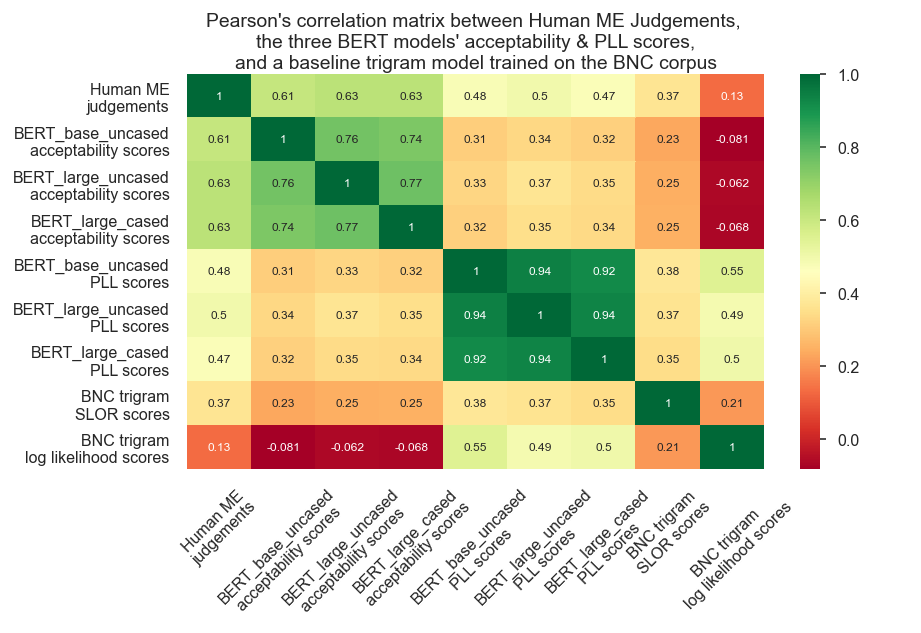
\includegraphics[scale=0.5]{templates/figures/bert_acc_pll_correlation_matrix.png}
    }
    \caption[PCC matrix between human judgements, BERT acceptability \newline \& PLL scores, and a trigram model]{PCC matrix between human judgements, BERT$_{\mathrm{CoLA}}$ acceptability scores, \& BERT$_{\mathrm{MLM}}$ PLL scores from all three BERT models.  In addition we add the SLOR and log likelihood scores of a trigram model trained on the British National Corpus by Sprouse et al. 2018 for additional reference.  All correlations shown have a $p$ < 0.0001.}
    \label{fig:bert_acc_pll_correlation_matrix}
\end{figure}


Additionally, we update our correlation graph from Figure \ref{fig:bert_acc_correlation_plot} in order to observe how the PLL scores may account for the full range of acceptability on an individual sentence level.

\begin{figure}[h!]
    %\centering
    \makebox[\textwidth][c]{
        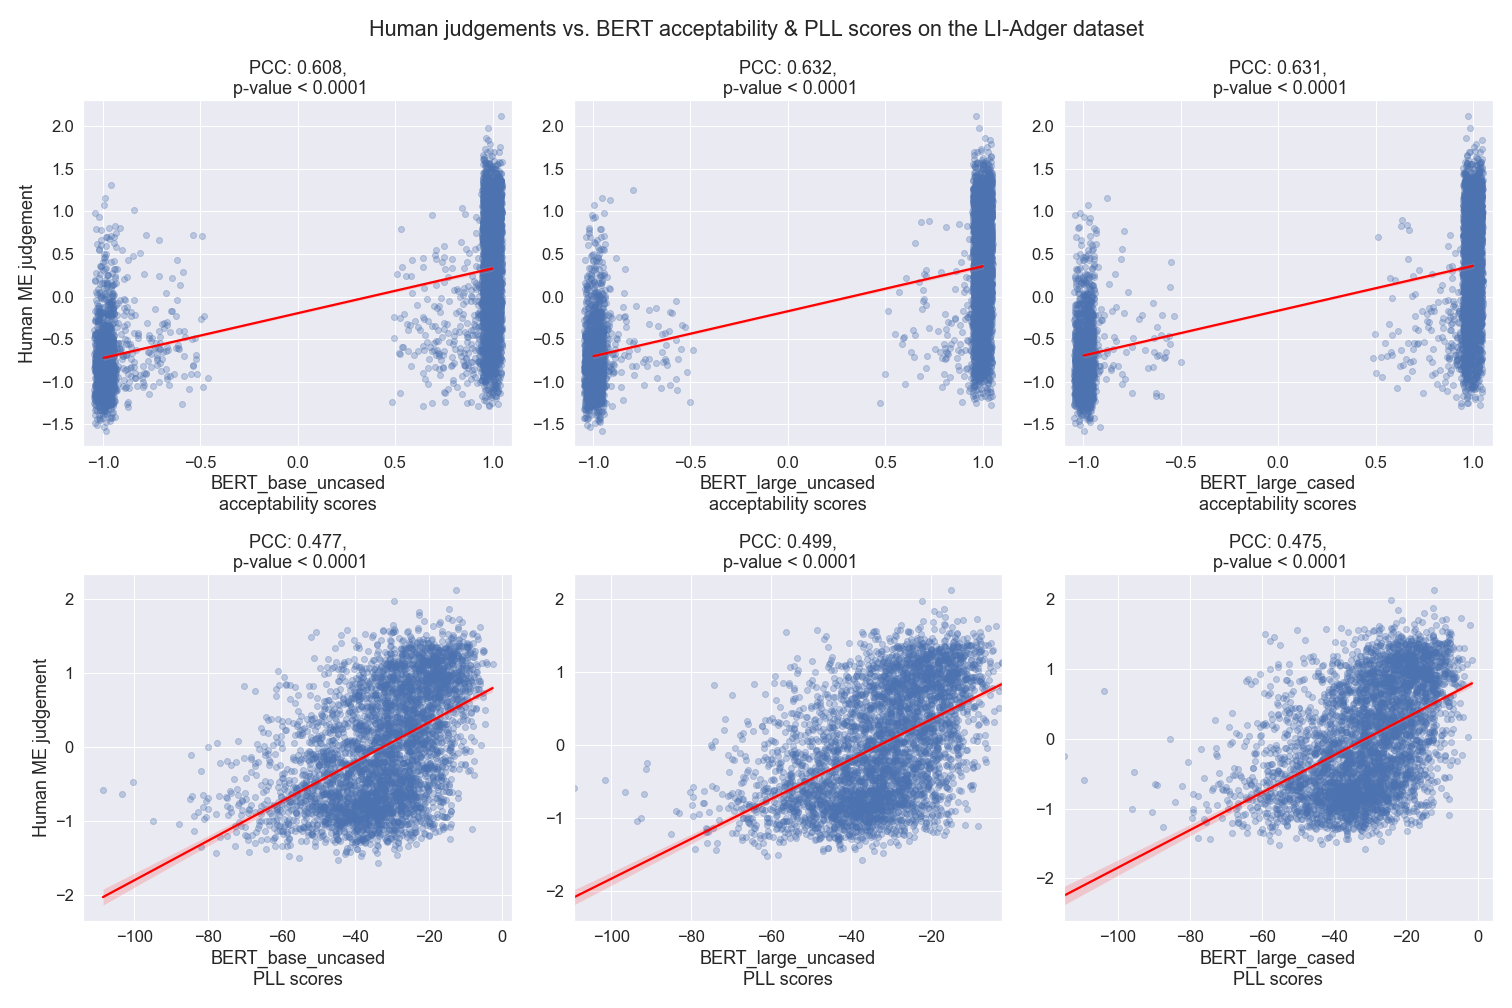
\includegraphics[scale=0.3]{templates/figures/bert_acc_pll_correlation_plot.png}
    }
    \caption[Human judgements vs. BERT acceptability \& PLL scores \newline on LI-Adger dataset]{Scatterplot of human judgements (y-axis) vs. BERT$_{\mathrm{CoLA}}$ acceptability scores, \& BERT$_{\mathrm{MLM}}$ PLL scores from all three BERT models for each sentence in the LI-Adger dataset with best-fit line in red.  We add a jitter of 0.05 along the x-axis and lower the alpha to 0.3 to highlight the density of the points.}
    \label{fig:bert_acc_pll_correlation_plot}
\end{figure}
\clearpage
If previous examples are on the mark, the fact that the PCCs for the BERT$_\mathrm{MLM}$ PLL scores are, on average, around 0.15 points lower than the corresponding BERT$_\mathrm{CoLA}$ acceptability scores is not indicative of performance on the ADC.  At least now with the PLL scores, the sentences truly seem to line up on a gradient scale, and one that appears to roughly track the best-fit line much better than the acceptability scores.  The next step is to calculate the PCCs for the Z-score transformed PLL deltas and add them to the correlation matrix in Figure \ref{fig:bert_acc_delta_correlation_matrix} in order to see how the PCCs change according to the more gradient metric.  We present in Figure \ref{fig:bert_acc_pll_delta_correlation_matrix} the updated correlation matrix comparing the baseline trigram model, BERT$_{\mathrm{CoLA}}$ acceptability delta scores and the newly calculated BERT$_{\mathrm{MLM}}$ PLL delta scores.

\begin{figure}[h]
    %\centering
    \makebox[\textwidth][c]{
        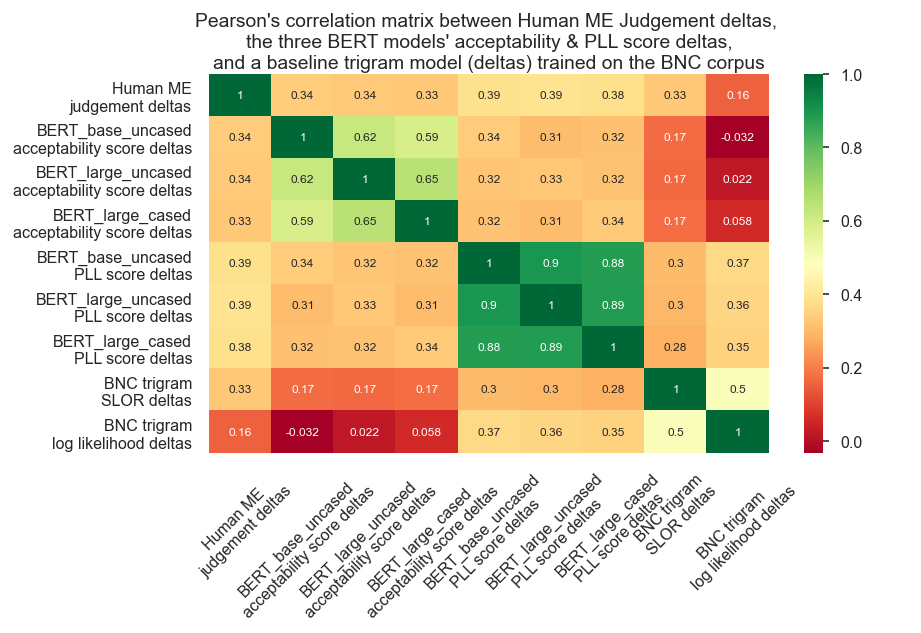
\includegraphics[scale=0.5]{templates/figures/bert_acc_pll_delta_correlation_matrix.png}
    }
    \caption[PCC matrix between human judgements, BERT$_{\mathrm{CoLA}}$,\newline BERT$_{\mathrm{MLM}}$, and a trigram model]{PCC matrix between human judgements and all three BERT$_{\mathrm{CoLA}}$ \& BERT$_{\mathrm{MLM}}$.  In addition we add the SLOR and log likelihood scores of a trigram model trained on the British National Corpus by Sprouse et al. 2018 for additional reference.  All correlations shown have a $p$ < 0.0001.}
    \label{fig:bert_acc_pll_delta_correlation_matrix}
\end{figure}

Encouragingly, we see a similar scenario to that of the trigram's SLOR score deltas and the three BERT$_{\mathrm{CoLA}}$s' acceptability score deltas discussed in Section \ref{section:2.5.1}.  Although the BERT$_{\mathrm{CoLA}}$s' acceptability scores at the individual sentence level obtain much higher PCCs with the human judgements on the LI-Adger dataset, that advantage disappears when calculating the PCCs between the human judgement deltas and the acceptability score deltas.  We see in Figure \ref{fig:bert_acc_pll_delta_correlation_matrix} that the PLL score deltas overtake the acceptability score deltas, although only by a small margin.  For completeness, we plot in Figure \ref{fig:bert_acc_pll_delta_correlation_plot} once more the correlation graphs in Figure \ref{fig:bert_acc_delta_correlation_plot} but adding the PLL score deltas to the comparison.
\begin{figure}[h]
    %\centering
    \makebox[\textwidth][c]{
        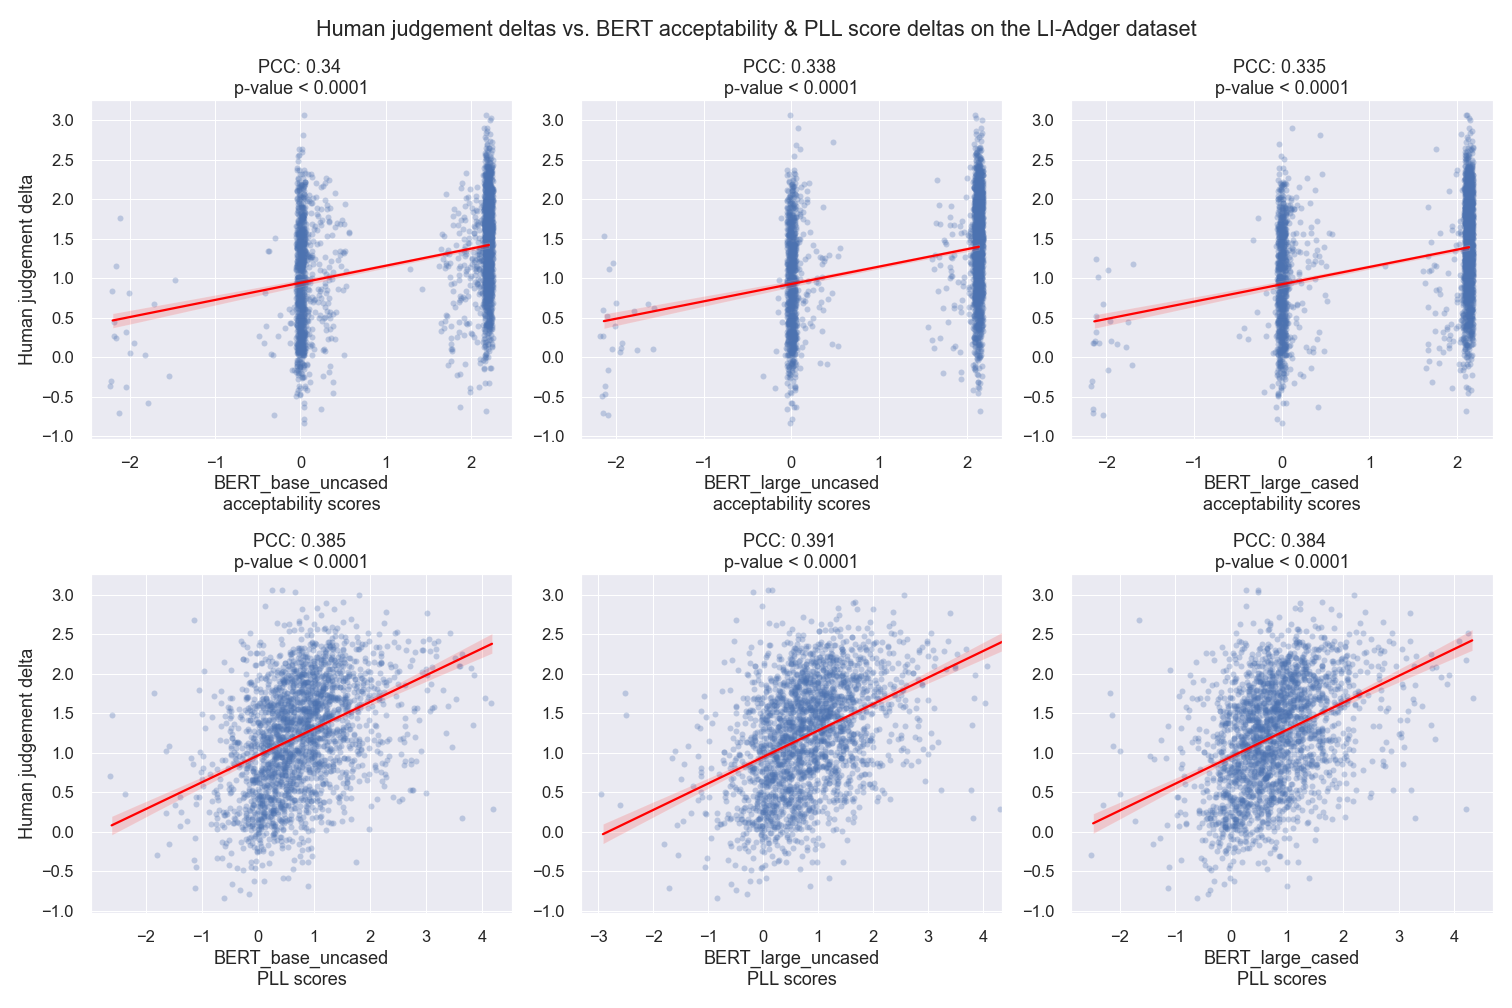
\includegraphics[scale=0.3]{templates/figures/bert_acc_pll_delta_correlation_plot.png}
    }
    \caption[Human judgements vs. BERT acceptability \& PLL scores \newline on LI-Adger minimal pairs]{Scatterplot of human judgement deltas (y-axis) vs. BERT$_{\mathrm{CoLA}}$ acceptability score delta \& BERT$_{\mathrm{MLM}}$ PLL delta for each minimal pair in the LI-Adger dataset with best-fit line in red.  We add a jitter of 0.05 along the x-axis and lower the alpha to 0.3 to highlight the density of the points.}
    \label{fig:bert_acc_pll_delta_correlation_plot}
\end{figure}

With all the preliminary correlations in place, we can set reasonable expectations for the BERT$_{\mathrm{MLM}}$ models' performance under the ADC using the PLL deltas.  We believe the gradience shown both at the sentence level PLL scores and the PLL deltas at the minimal pair level will yield better performance under the ADC at all three levels tested ($\delta=0.5$, $\delta=1.0$ and $\delta=5.0$).  How much better that performance is, remains to be seen.

\section{BERT says best 2 out of 3 (ADC round 2)}
Similar to Section \ref{section:2.5.2}, we apply the BLiMP Criterion and the ADC with $\delta=\{0.5, 1.0, 5.0\}$ in order to see how the ADC scales as it becomes less strict and generalizes to a form similar to the BLiMP Criterion.  We report the performance of the three BERT$_{\mathrm{MLM}}$ models using their PLL scores along with all the previously evaluated models in Table \ref{tab:table_15}.
\begin{table}[h]
    \centering
    \ra{1.3}
    \begin{tabular}{@{}lcccc@{}}
    \toprule
    \textbf{Model} & \textbf{BLiMP} & \textbf{ADC, $\delta=0.5$} & \textbf{ADC, $\delta=1.0$} & \textbf{ADC, $\delta=5.0$}  \\
    \midrule
    BERT$_{base-uncased; \mathrm{MLM}}$ & 0.852 & 0.364 & 0.631 & 0.849 \\
    BERT$_{large-uncased; \mathrm{MLM}}$ & 0.866 & 0.378 & 0.658 & 0.859 \\
    BERT$_{large-cased; \mathrm{MLM}}$ & 0.871 & 0.376 & 0.661 & 0.868 \\
    \midrule
    BERT$_{base-uncased; \mathrm{CoLA}}$ & 0.915 & 0.286 & 0.538 & 0.902 \\
    BERT$_{large-uncased; \mathrm{CoLA}}$ & 0.917 & 0.311 & 0.564 & 0.907 \\
    BERT$_{large-cased; \mathrm{CoLA}}$ & 0.936 & 0.307 & 0.561 & 0.925 \\
    \midrule
    trigram$_{SLOR}$ & 0.753 & 0.301 & 0.520 & 0.744\\
    trigram$_{log-prob}$ & 0.671 & 0.165 & 0.329 & 0.668 \\
    \bottomrule
    \end{tabular}
    \caption[BERT$_{\mathrm{MLM}}$, BERT$_{\mathrm{CoLA}}$, and trigram model scores\newline under BLiMP \& ADC]{Comparison between the models' BLiMP and ADC scores, using $\delta$=\{0.5, 1.0, 5.0\}. We include three BERT$_{\mathrm{MLM}}$ models, three BERT$_{\mathrm{CoLA}}$ models, as well as SLOR and log-likelihood scores from a trigram model trained on the British National Corpus by Sprouse et al. 2018}
    \label{tab:table_15}
\end{table}

Reassuringly, the higher PCCs shown in Figures \ref{fig:bert_acc_pll_delta_correlation_matrix} and \ref{fig:bert_acc_pll_delta_correlation_plot} by the BERT$_{\mathrm{MLM}}$ models' PLL output translate well to better performance than the BERT$_{\mathrm{CoLA}}$ models on the ADC for $\delta=0.5$ and $\delta=1.0$.  However, when the distance between the models' output deltas and the human judgement deltas (Equation \ref{eqn:acceptability_delta_criterion_b}) is no longer considered by the ADC ($\delta=5.0$), the BERT$_{\mathrm{CoLA}}$ models outperform the BERT$_{\mathrm{MLM}}$ models.  This is likely due to the lack of gradience in the BERT$_{\mathrm{CoLA}}$ models' acceptability output no longer being a determining factor in whether they evaluated a minimal pair correctly or not. This is presented in more detail below. First, as in Section \ref{section:2.5.2}, we inspect 4 minimal pairs where the BERT$_{\mathrm{MLM}}$ models meet the BLiMP Criterion but not the ADC with a $\delta=5.0$, shown in Table \ref{tab:table_16}.  

\begin{table}[h]
    \centering
    \ra{1.3}
    \begin{tabular}{@{}lcc@{}}
    \toprule
    \textbf{Minimal Pair} & Human & BERT$_{\mathrm{MLM}}$\\
    \textbf{Top}: Acceptable | \textbf{Bottom}: Unacceptable & judgement & PLL\\
    \toprule
    What is there a coupon for on the counter?  & 0.085185 & 0.731265 \\
    *What is a coupon for on the counter? & 0.134364 & 0.00874871 \\
    \midrule
   What the runners believe is that they will win the race. & -0.23705 &  1.44651 \\
    *What the runners believe is they will win the race. &  -0.1155 & 1.1792 \\
    \midrule
    I guessed he was married. & 0.111685 & 1.3683 \\
    *I guessed he is married.  &  0.588843	 & 0.753377 \\
    \midrule
    The announcer's introduction of Ted was humorous.  & 0.659471 & 0.52595 \\
    *The announcer's introduction of Ted's was humorous. & 0.748718 & 0.378315 \\
    \bottomrule
    \end{tabular}
    \caption[Four minimal pairs where BERT$_{\mathrm{MLM}}$ meets the BLiMP\newline Criterion but not the ADC with $\delta=5.0$]{Four minimal pairs where all 3 models BERT$_{\mathrm{MLM}}$ passed the BLiMP criterion but not the generalized ADC with $\delta=5.0$. We report the BERT$_{\mathrm{MLM}}$ PLL scores from BERT$_{\mathrm{MLM}_{\mathrm{large-cased}}}$. The human judgement and BERT$_{\mathrm{MLM}}$ PLL scores are already z-score transformed.}
    \label{tab:table_16}
\end{table}

Although the three BERT$_{\mathrm{MLM}}$ models failed to meet the ADC with $\delta=5.0$ in Table \ref{tab:table_16}, the reported PLL scores from BERT$_{\mathrm{MLM}_{\mathrm{large-cased}}}$ immediately show how BERT$_{\mathrm{MLM}}$'s PLL scores are much more gradient than the acceptability outputs from the BERT$_{\mathrm{CoLA}}$ models.  Let us inspect a few more example minimal pairs, but this time those where the BERT$_{\mathrm{MLM}}$ models met the ADC with $\delta=5.0$ but not the BLiMP Criterion, shown in Table \ref{tab:table_17}.

\begin{table}[h]
    \centering
    \ra{1.3}
    \begin{tabular}{@{}lcc@{}}
    \toprule
    \textbf{Minimal Pair} & Human & BERT$_{\mathrm{MLM}}$\\
    \textbf{Top}: Acceptable | \textbf{Bottom}: Unacceptable & judgement & PLL\\
    \toprule
    We proved Amelia to the manager to be responsible.  & -0.56008 & -1.77701 \\
    *We proved to the manager Amelia to be responsible. & -0.13864 & -1.26881 \\
    \midrule
    What did you give to whom? & 0.082244 & 0.899228 \\
    *To whom did you give what? & 0.289657 & 0.930362 \\
    \midrule
    There is likely to depart a train at midnight. & -0.53097 & -0.706574 \\
    *There is likely a train to depart at midnight.  &  0.177497 & 0.441587 \\
    \midrule
    Jenny would accurately have calculated the results. & 0.345683 & -1.90655 \\
    *Jenny accurately will calculate the results.  & 0.501494 & -0.458686 \\
    \bottomrule
    \end{tabular}
    \caption[Four minimal pairs where BERT$_{\mathrm{MLM}}$ meets the ADC\newline with $\delta=5.0$ but not the BLiMP Criterion]{Four minimal pairs where all 3 BERT$_{\mathrm{MLM}}$ models pass the generalized ADC with $\delta=5.0$ but not the BLiMP criterion. We report the BERT$_{\mathrm{MLM}}$ PLL scores from BERT$_{\mathrm{MLM}_{\mathrm{large-cased}}}$. The human judgement and BERT$_{\mathrm{MLM}}$ PLL scores are already z-score transformed.}
    \label{tab:table_17}
\end{table}

What all the example minimal pairs in Table \ref{tab:table_17} have in common is that the human judgements disagree with the expert labels.  Therefore, if we were to evaluate the human judgements themselves under the BLiMP Criterion, they would not pass either.  However, reading the second and third minimal pair in Table \ref{tab:table_17} highlights precisely why it is preferable to rely on human judgements before the expert labels: those two minimal pairs are very close in acceptability values, and in fact read almost the same to native speakers.  This additional resolution is lost when switching to categorical expert labels such as those required by BLiMP.  The BERT$_{\mathrm{MLM}}$ PLL scores agree in monotonicity with the human judgements too; that is, the three BERT$_{\mathrm{MLM}}$ models scored the unacceptable sentence in the minimal pair higher than the acceptable sentence, following the trend in the human judgements for the four examples in Table \ref{tab:table_17}.  Unfortunately, this is not a consistent trend.  For example, upon inspection of a few examples where the BERT$_{\mathrm{CoLA}}$ models meet the generalized ADC ($\delta=5.0$) but not the BERT$_{\mathrm{MLM}}$ models, we see the added gradience of the PLL scores alone is not enough.  The four examples in Table \ref{tab:table_18} show the BERT$_{\mathrm{CoLA}}$ models follow the monotonicity of the human judgements, whilst the BERT$_{\mathrm{MLM}}$ models flip which sentence is the more acceptable of the pair.  Under $\delta=5.0$, the lack of gradience no longer affects the BERT$_{\mathrm{CoLA}}$ models, thus allowing them to finally score higher than the BERT$_{\mathrm{MLM}}$ models, which they were unable to do for $\delta=0.5$ nor $\delta=1.0$.  However, there are cases where, even with $\delta=5.0$, BERT$_{\mathrm{MLM}}$ scores minimal pairs correctly that BERT$_{\mathrm{CoLA}}$ is unable to account for, show in Table \ref{tab:table_19}.

\begin{table}[h]
    \centering
    \ra{1.3}
    \begin{tabular}{@{}lccc@{}}
    \toprule
    \textbf{Minimal Pair}                                    & Human & BERT$_{\mathrm{CoLA}}$   & BERT$_{\mathrm{MLM}}$ \\
    \textbf{Top}: Acceptable | \textbf{Bottom}: Unacceptable & judgement & acceptability      & PLL\\
    \toprule
    The book was written truthfully.  & 1.30085 & 0.732642 & 1.00074 \\
    *The book writes truthfully. & -0.40842 & -1.40058 & 1.03895 \\
    \midrule
    It stormed suddenly. & 0.548385 & -1.39038 & 0.506643 \\
    *It suddenly stormed.    & 0.451832 &  -1.39582 & 0.785855 \\
    \midrule
    How few people were there at the rally? & 0.371244 & 0.732758 & 0.989334 \\
    *How few people there were at the rally? & -0.01639 & 0.732748 & 1.02265 \\
    \midrule
    The IRS denied Lilly her refund.  & 1.40233 & 0.732951 & -1.22485 \\
    *The IRS denied her refund to Lilly. & -0.47087 & 0.612725 & -0.966726 \\
    \bottomrule
    \end{tabular}
    \caption[Four minimal pairs where BERT$_{\mathrm{CoLA}}$ meets ADC \newline with $\delta=5.0$ but the BERT$_{\mathrm{MLM}}$ models do not]{Four minimal pairs where all BERT$_{\mathrm{CoLA}}$ models meet the ADC with $\delta=5.0$ but the BERT$_{\mathrm{MLM}}$ models do not. We report the scores from BERT$_{large-cased}$. The human judgement, acceptability, and PLL scores are already z-score transformed. }
    \label{tab:table_18}
\end{table}

\begin{table}[h]
    \centering
    \ra{1.3}
    \begin{tabular}{@{}lccc@{}}
    \toprule
    \textbf{Minimal Pair}                                    & Human & BERT$_{\mathrm{CoLA}}$   & BERT$_{\mathrm{MLM}}$\\
    \textbf{Top}: Acceptable | \textbf{Bottom}: Unacceptable & judgement & acceptability      & PLL\\
    \toprule
    Toby said to Sally to take care of herself.  & 0.188154 & -1.39838
 & 0.540271 \\
    *Toby said to Sally to take care of himself. & -0.488670 & 0.608852 & 0.348782 \\
    \midrule
    I predicted she was guilty.  & 0.703876 & 0.730575 & 0.615354 \\
    *I predicted she may be guilty.	 & 0.530117 &  0.732155 & 0.18414 \\
    \midrule
    The ice melted quickly on the table. & 1.459752	 & 0.729108 & 1.34043 \\
    *The ice quickly melted on the table. & 0.618948 & 0.730474 & 1.18234 \\
    \midrule
    A lawyer smarter than my brother...  & 0.596167 & 0.733196 & -0.188386 \\
    *A smarter lawyer than my brother... & 0.782106 & 0.733102 & 0.123958 \\
    \bottomrule
    \end{tabular}
    \caption[Four minimal pairs where BERT$_{\mathrm{MLM}}$ meets ADC\newline with $\delta=5.0$ but BERT$_{\mathrm{MLM}}$ does not]{Four minimal pairs where all BERT$_{\mathrm{MLM}}$ models meet the ADC with $\delta=5.0$ but not the BERT$_{\mathrm{CoLA}}$ models. We report the scores from BERT$_{large-cased}$. The human judgement, acceptability, and PLL scores are already z-score transformed. }
    \label{tab:table_19}
\end{table}
\clearpage
%\todo[inline]{Bob asks why using the surrounding context of the masked token is in principle similar to the ngram}

Our analyses of the BERT$_{\mathrm{MLM}}$ models continue by conducting the same trigram-overlap analyses we did with the BERT models fine-tuned using CoLA.  \textit{A priori} there likely is a much larger overlap between the trigram model's SLOR predictions and BERT$_{\mathrm{MLM}}$'s PLL predictions by the very nature of the MLM procedure.  BERT$_{\mathrm{MLM}}$ uses the surrounding context of a masked token to predict a probability distribution $P(w_j|w_0,...,w_{j-1},w_{j+1},...w_n)$ (Equation \ref{eqn:mlm_token_prob_b}) for each token in a given sequence of words $s_i$.  This is, in principle, similar to a trigram using the preceding context of a word to predict its likelihood $P(w_j|w_{j-3},w_{j-2},w_{j-1})$.  We say \textit{in principle} because the MLM and $N$-gram outputs and training regimes can be framed in terms of predicting individual tokens given their context, with the caveat that the trigram is severely handicapped in terms of the machinery it has at its disposal.  However, BERT$_{\mathrm{CoLA}}$ outputs a probability distribution over a finite set of categorical labels when given the entire sequence $s_i$ as input, so it is much farther removed from the computations a trigram performs relative to BERT$_{\mathrm{MLM}}$.  We assess the extent of this similarity by calculating the ADC for $\delta=0.5$ and $\delta=1.0$ once again.  Then for each value of $\delta$, we create a new dataset by subtracting the minimal pairs from LI-Adger dataset that were correctly predicted by the trigram's SLOR scores.  We finalize by recalculating the BERT$_{\mathrm{MLM}}$ models' ADC scores using the reduced datasets.  The results for the procedure are presented in Table \ref{tab:table_20}.

%\begin{table}[h]
    %\centering
    %\ra{1.3}
    %\begin{tabular}{@{}cccc@{}}
    %\toprule
    %\textbf{Model} & \textbf{ADC, $\delta=0.5$} & \textbf{ADC, %$\delta=0.5$} & \textbf{Total} \\
                   %& \textbf{original}          & \textbf{sans trigram}      & \textbf{overlap}\\
    %\midrule
    %BERT$_{base-uncased; \mathrm{MLM}}$ & 0.364 & 0.323 & 13.87\% \\
    %BERT$_{large-uncased; \mathrm{MLM}}$ & 0.378 & 0.333 & 14.50\% \\
    %BERT$_{large-cased; \mathrm{MLM}}$ & 0.376 & 0.335 & 14.21\% \\
    %\bottomrule
    %\end{tabular}
    %\caption[MLM-objective BERT models' ADC with $\delta=0.5$ scores sans easy min pairs]{MLM-objective BERT models' performance on the ADC with $\delta=0.5$ before and after removing all minimal pairs for which the ADC Criterion was met by the trigram baseline model trained on the BNC corpus. The third column is the percentage of BERT's passing minimal pairs that the trigram baseline also passed.}
    %\label{tab:xxxxx}
%\end{table}

%\begin{table}[h]
    %\centering
    %\ra{1.3}
    %\begin{tabular}{@{}cccc@{}}
    %\toprule
    %\textbf{Model} & \textbf{ADC, $\delta=1.0$} & \textbf{ADC, %$\delta=0.5$} & \textbf{Total} \\
                   %& \textbf{original}          & \textbf{sans trigram}      & \textbf{overlap}\\
    %\midrule
    %BERT$_{base-uncased; \mathrm{MLM}}$ & 0.631 & 0.553 & 36.58\% \\
    %BERT$_{large-uncased; \mathrm{MLM}}$ & 0.658 & 0.586 & 37.51\% \\
    %BERT$_{large-cased; \mathrm{MLM}}$ & 0.661 & 0.589 & 37.80\% \\
    %\bottomrule
    %\end{tabular}
    %\caption[MLM-objective BERT models' ADC with $\delta=1.0$ scores sans easy min pairs]{MLM-objective BERT models' performance on the ADC with $\delta=1.0$ before and after removing all minimal pairs for which the ADC Criterion was met by the trigram baseline model trained on the BNC corpus. The third column is the percentage of minimal pairs that both the BERT model and the trigram baseline pass.}
    %\label{tab:xxxxxxx}
%\end{table}

\begin{table}[h!]
    \centering
    \ra{1.3}
    \begin{tabular}{@{}lcccccc@{}}
    \toprule
    \textbf{Model} & \multicolumn{3}{c}{\textbf{ADC, $\delta=0.5$}} &  \multicolumn{3}{c}{\textbf{ADC, $\delta=1.0$}} \\
    \cmidrule{2-3} \cmidrule{4-7}
    \textbf{BERT}$_\mathrm{MLM}$ & \textbf{Original} & \textbf{Reduced} & \textbf{Overlap} & \textbf{Original} & \textbf{Reduced} & \textbf{Overlap} \\
    \midrule
    base-uncased & 0.364 & 0.323 & 13.87\% & 0.631 & 0.553 & 36.58\%\\
    large-uncased & 0.378 & 0.333 & 14.50\% & 0.658 & 0.586 & 37.51\%\\
    large-cased & 0.376 & 0.335 & 14.21\% &  0.661 & 0.589 & 37.80\% \\
    \bottomrule
    \end{tabular}
    \caption[BERT$_{\mathrm{MLM}}$ ADC with $\delta=$\{0.5,1.0\} scores\newline sans easy min pairs]{BERT$_{\mathrm{MLM}}$ models' performance on the ADC with $\delta$={0,5,1.0} before (Original) and after (Reduced) removing all minimal pairs for which the ADC Criterion was met by the trigram baseline model trained on the BNC corpus. The Overlap columns display the percentage of minimal pairs that both the BERT$_{\mathrm{MLM}}$ model and the trigram baseline pass.}
    \label{tab:table_20}
\end{table}

A difference that becomes immediately apparent is the drop in total performance across the board for all three BERT$_{\mathrm{MLM}}$ models both for $\delta=0.5$ and $\delta=1.0$ once the minimal pairs correctly scored by the trigram are removed from the dataset.  Unsurprisingly, the percentage of the minimal pairs scored correctly by both BERT$_{\mathrm{MLM}}$ and the trigram SLOR model correctly is on average 14.2\% for $\delta=0.5$ (up from 8.8\% with BERT$_{\mathrm{CoLA}}$) and 37.3\% for $\delta=1.0$ (up from 28.8\% with BERT$_{\mathrm{CoLA}}$).

Finally, this brings us to the question posed at the end of Chapter \ref{chapter:chapter2}: What is lost (or gained) in terms of performance under the ADC by switching from  BERT$_{\mathrm{CoLA}}$ acceptability scores to BERT$_{\mathrm{MLM}}$ PLL scores?  We present in Table \ref{tab:table_22} the performance of BERT$_{\mathrm{MLM}}$ under the ADC as shown previously, but add an additional column containing the percentage of overlap between BERT$_{\mathrm{MLM}}$ and BERT$_{\mathrm{CoLA}}$, i.e. what percentage of the minimal pairs in the LI-Adger dataset was classified correctly by both BERT models.  We carry out this calculation for $\delta=0.5$ and $\delta=1.0$ as with the trigrams assessment because these are where ADC enforces the gradient aspect of the minimal pairs, not just their monotonicity.

\begin{table}[h!]
    \centering
    \ra{1.3}
    \begin{tabular}{@{}lcccc@{}}
    \toprule
    \textbf{Model} & \multicolumn{2}{c}{\textbf{ADC, $\delta=0.5$}} &  \multicolumn{2}{c}{\textbf{ADC, $\delta=1.0$}} \\
    \cmidrule{2-3} \cmidrule{4-5}
    \textbf{BERT}$_{\mathrm{MLM}}$ & \textbf{Score} & \textbf{Overlap} & \textbf{Score} & \textbf{Overlap}  \\
    \midrule
    base-uncased & 0.364 & 9.05\% & 0.631 & 34.25\% \\
    large-uncased & 0.378 & 9.73\% & 0.658 & 37.29\% \\
    large-cased & 0.376 & 9.89\% & 0.661 & 37.04\% \\
%    \midrule
%    BERT$_{base-uncased; \mathrm{CoLA}}$ & 0.286 & 9.05\% & 0.538 & 34.25\% \\
%    BERT$_{large-uncased; \mathrm{CoLA}}$ & 0.311 & 9.73\% & 0.564 & 37.29\% \\
%    BERT$_{large-cased; \mathrm{CoLA}}$ & 0.307 & 9.89\% & 0.561 & 37.04\% \\
    \bottomrule
    \end{tabular}
    \caption[Overlap between BERT$_{\mathrm{MLM}}$ and BERT$_{\mathrm{CoLA}}$ under the ADC]{The percentage of minimal pairs that both BERT$_{\mathrm{MLM}}$ and BERT$_{\mathrm{CoLA}}$ passed, as well as the ADC scores with $\delta$=\{0.5, 1.0\} of the BERT$_{\mathrm{MLM}}$ models for reference.}
    \label{tab:table_22}
\end{table}

The overlap between BERT$_{\mathrm{MLM}}$ and BERT$_{\mathrm{CoLA}}$, although substantial, only accounts for roughly one third of the minimal pairs either of the two models scored correctly under the stricter $\delta=0.5$ measure.  Relaxing the ADC to $\delta=1.0$ allows the overlap between the two models to account for roughly half of the minimal pairs they each scored correctly.  However, this supports the interpretation we set out to test at the beginning of this chapter: BERT$_{\mathrm{MLM}}$ and BERT$_{\mathrm{CoLA}}$ behave almost completely differently, even demonstrating different KoL despite relying on the same pretrained BERT model.  Training an additional classifier on top of BERT, as we did with CoLA, further obfuscates any information to be gained from conducting an input-output analysis on the model.

%\section{A successful maiden voyage for ADC}


%Using the BERT$_{\mathrm{CoLA}}$ and 


%The lack of gradience demonstrated by the BERT models fine-tuned using the CoLA training set provided the optimal 






%% This is an example contributions chapter.  You should put chapter/appendix that you
%% write into a separate file, and add a line \include{yourfilename} to
%% main.tex, where `yourfilename.tex' is the name of the chapter/appendix file.
%% You can process specific files by typing their names in at the 
%% \files=
%% prompt when you run the file main.tex through LaTeX.
\chapter*{Contributions}
\addcontentsline{toc}{chapter}{Contributions}

This thesis has reviewed current empirical methods of assessing the KoL of LMs, and found that to date there exists no test of KoL that is comprehensive in its coverage of linguistic phenomena, is backed by attested and replicable human judgement data, and tests LMs' ability to track different linguistic phenomena across the full range of the acceptability gradient.  This thesis addresses this gap by proposing the three necessary components needed to construct such a comprehensive test of KoL.

First, this thesis presents the LI-Adger dataset, a collection of 150 pairwise phenomena collected by Sprouse et al. (2013) from Linguistic Inquiry (LI) 2001-2010, and an additional 105 multi-condition phenomena collected by Sprouse \& Almeida (2012) from an exhaustive selection of 219 sentence types from Adger's (2003) \textit{Core Syntax} textbook.  The phenomena represented in the LI-Adger dataset far exceed the coverage of the most recent datasets published to date for the purposes of testing the KoL in LMs.  The Corpus of Linguistic Acceptability (CoLA; Warstadt \& Bowman 2019) and The Benchmark of Linguistic Minimal Pairs for English (BLiMP; Warstadt et al. 2020).

This thesis supports the LI-Adger dataset with statistically powerful, replicable and validated human Magnitude Estimate (ME) data collected by Sprouse et al (2013) and Sprouse \& Almeida (2012).  The data accompanying the LI dataset boasts a 95 percent $\pm5$ minimum replication rate (Sprouse et al. 2013), whereas the ME data in the Adger dataset increases the minimum replication rate to over 97\% (Sprouse \& Almeida 2012)..  Additionally, Sprouse et al. (2018) determined the statistical power of both the LI and Adger datasets to meet the 80\% power threshold for the detection of False Negatives.

This dataset and accompanying human judgements then become the gold standard in terms of coverage and reliability.  In order to make full use of this dataset, this thesis proposes the Acceptability Delta Criterion, a metric that tests LMs for Human KoL by enforcing the gradience of acceptability and requiring LMs to track the validated human judgements through the gradient spectrum as the acceptability values change across minimal pairs.  We demonstrate further that adopting a functionally categorical view of acceptability leads to an unstable BERT model when fine-tuned with CoLA achieving 94\% correct classification of the minimal pairs in the LI-Adger dataset; while a trigram model trained on the British National Corpus (BNC) by Sprouse et al. 2018 achieves (75\%).  These results imply that either trigram models are able to account for 75\% of the phenomena in Generative grammar, or, alternatively, that treating acceptability as a categorical metric leads to a high false positive rate in KoL tests.  Accordingly, the ADC with a strict $\delta=0.5$ determined that neither BERT, whose predictions were nearly all categorical, and the trigram model both only correctly accounted for roughly 30\% of the minimal pairs in the LI-Adger dataset.  Using the defaul BERT models with gradient \textit{pseudo log-likelihood} (PLL) outputs increased its score to (37\%), further demonstrating the need for gradience in order to meet the ADC.

The three main contributions of this thesis when used together create the most comprehensive test of Human KoL for LMs currently available.  With further ongoing work, the test will also allow us to see a fine-grained analysis of which phenomena a LM was able to account for in its output and how well it predicted the acceptability judgements around them.  It is to be hoped that researchers will adopt the LI-Adger dataset for its coverage of Generative grammar and rely on the human judgements as the ground-truth labels that LMs are expected to approximate, and, beyond that, the ADC.
\appendix
%% This defines the bibliography file (main.bib) and the bibliography style.
%% If you want to create a bibliography file by hand, change the contents of
%% this file to a `thebibliography' environment.  For more information 
%% see section 4.3 of the LaTeX manual.
\begin{singlespace}
\bibliography{main}
\bibliographystyle{newapa}
\end{singlespace}

\end{document}

